\documentclass[a4paper, 12pt]{report}
\usepackage[utf8]{inputenc}
\usepackage[T2A]{fontenc}
\usepackage[english,russian]{babel}
\usepackage[dvips]{graphicx}
\usepackage[left = 2cm, top = 1cm, right = 2cm, bottom = 2cm]{geometry}
\usepackage{hyperref}
% \usepackage{xcolor}
\usepackage{titlesec}
\usepackage{listings}
\usepackage{amssymb,amsmath,amsthm}
\usepackage{enumerate}
\usepackage[all]{xy}

\usepackage{color}

\usepackage{shortcuts}

\newtheorem{definition}{Определение}[chapter]
\newtheorem{theorem}{Теорема}
\newtheorem{St}{Утверждение}[chapter]

\lstloadlanguages{C,[ANSI]C++}%,Clean,make,Fortran}%Загружаемые языки
\lstset{extendedchars=false,
        breaklines=true, %автоперенос длинных линий
        breakatwhitespace=true}
\graphicspath{{pic/}}
\titleformat{\chapter}[block]{\color{black}\Large\bfseries\filcenter}{}{1em}{}
\setcounter{secnumdepth}{0}


\begin{document}
\title{Основания алгебраического подхода к синтезу корректных алгоритмов}
\author{Лектор~--- Рудаков К.В.\\ Наборщик~--- Старожилец В.М.\\ Редактор~--- Рыскина М. Н.}
\date{}
\maketitle

\tableofcontents

\chapter{Лекция 1}
\section{Введение}
Данные лекции рассматривают общую задачу машинного обучения без привязки к конкретным методам и основы алгебраического подхода к синтезу корректных алгоритмов для её решения. В некотором роде они являются взглядом сверху на задачи машинного обучения и методы их решения.

В первую очередь следует сформулировать задачу машинного обучения в общем виде. По сути это задача построения алгоритма, который реализует отображение из множества начальных информаций в множество конечных информаций. Сразу отметим, что в курсе рассматриваются только такие отображения, для которых существует реализующий их алгоритм.

\begin{definition}
Символом $\mathfrak{I_i}$ (читается <<И инишл>>) будем обозначать множество начальных информаций, например, симптомы болезни.
\end{definition}

\begin{definition}
Символом $\mathfrak{I_f}$ (читается <<И файнэл>>) будем обозначать множество конечных информаций, например, диагноз.
\end{definition}

Таким образом, на формальном языке нам требуется найти такой алгоритм $A$, что он осуществляет отображение из множества начальных информаций $\mathfrak{I_i}$ в множество конечных информаций $\mathfrak{I_f}$:
\[
A: \mathfrak{I_i} \rightarrow \mathfrak{I_f}.
\]
Пока что задача поставлена так, что нам нужно найти некоторое произвольное отображение из одного множества в другое, реализуемое некоторым алгоритмом. При этом свойства этого отображения и алгоритма неважны. В такой постановке у нас нет каких-либо ограничений на искомый алгоритм: даже датчик случайных чисел является решением этой задачу. Поэтому вводятся дополнительные ограничения на допустимые алгоритмы. Итак,

\begin{definition}
Обозначим $\mathfrak{M}^* = \{A|\ A:\  \mathfrak{I_i}\rightarrow \mathfrak{I_f}\}$ множество всех алгоритмов, реализующих отображение из $\mathfrak{I_i}$ в $\mathfrak{I_f}$.
\end{definition}

\begin{definition}
Обозначим $I_{str}$ структурную информацию, содержащую условия и требования, накладываемые на $A$.
\end{definition}

\begin{definition}
Обозначим $\mathfrak{M}(I_{str}) \subset \mathfrak{M}^*$ некоторое подмножество $\mathfrak{M}^*$, удовлетворяющее $I_{str}$.
\end{definition}

Теперь у нас есть дополнительная информация $I_{str}$, позволяющая накладывать дополнительные ограничения на нашу задачу. Введём определения допустимого отображения и корректного алгоритма.

\begin{definition}
Любое отображение из множества $\mathfrak{M}(I_{str})$ называется допустимым.
\end{definition}

\begin{definition}
Задача Z заключается в построении алгоритма, реализующего допустимое отображение.
\end{definition}

\begin{definition}
Любой алгоритм, реализующий любое допустимое отображение, называется корректным.
\end{definition}

В такой формулировке необходимым и достаточным условием разрешимости задачи Z является выполнение выражения:
\[
\mathfrak{M}(I_{str}) \neq \emptyset,
\]
а условием единственности решения~--- выполнение равенства:
\[
|\mathfrak{M}(I_{str})| = 1.
\]
Заметим также, что в данной формулировке корректный алгоритм~--- это алгоритм, не допускающий ни одной ошибки, а множество $\mathfrak{M}(I_{str})$~--- множество алгоритмов не допускающих ошибок. Однако можно поставить условия несколько мягче, и дать алгоритмам возможность ошибаться.

\section{Поиск решения задачи}
Пусть $\mathfrak{M}(\pi)$~--- некоторое параметрическое семейство отображений. После того как мы выбрали некоторое семейство отображений $\mathfrak{M}(\pi)$, попытаемся попасть в $\mathfrak{M}(I_{str})$, взяв в $\mathfrak{M}(\pi)$ какое-нибудь отображение за начальное. Это возможно, если данные семейства пересекаются:
\[
\mathfrak{M}(\pi) \cap \mathfrak{M}(I_{str}) \neq \emptyset.
\]

Но, с одной стороны, чем \emph{сложнее} наше семейство, тем выше вероятность, что оно пересекается с семейством $\mathfrak{M}(I_{str})$, однако, с другой стороны, достижение этого пересечения может быть \emph{затратно}, если $\mathfrak{M}(\pi)$ сложное. Также всегда остаётся вероятность, что множество $\mathfrak{M}(\pi)$ с $\mathfrak{M}(I_{str})$ не пересекается. Для поиска компромиссного решения используют идею \emph{расширения множества}.

\begin{definition}
Пусть $f$~--- некоторая операция над множеством $\mathfrak{M}^*$. Тогда $f(\mathfrak{M}(\pi))$ будем называть расширением множества $\mathfrak{M}(\pi)$.
\end{definition}

Таким образом, мы хотим расширить некоторое <<простое>> множество до пересечения с $\mathfrak{M}(I_{str})$. Однако, не любая функция $f$ нам подходит, так как <<простое>> множество может расшириться до слишком <<сложного>> множества. Важно, что $f$ мы выбираем сами, поэтому можем выбрать его так, чтобы искать нужный алгоритм было не слишком сложно.

\chapter{Лекция 2}
\section{Алгебра, реляционная система и алгебраическая система}
Данная лекция посвящена вопросам терминологии, используемой в данном курсе. Поэтому тут будет очень много определений (ещё больше, чем в предыдущей). Для начала определим понятия алгебры, реляционной системы и алгебраической системы.

\begin{definition}
Сигнатура~--- набор характеристик, однозначно идентифицирующих объект.
\end{definition}

\begin{definition}
Отношение~--- математическая структура, которая формально определяет свойства различных объектов и их взаимосвязи. В нашем курсе будет обозначаться буквой $R$, то есть
\[
R: A^n \rightarrow \{ 0, 1 \}
\]
\end{definition}
Отношение $R$ принимает на вход $n$ элементов множества $A$ и проверяет выполняется ли свойство, задаваемое отношением. Например, свойство делимости, равенства и т.д.

\begin{definition}
Операцией $Op$ называется следующее отображение:
\[
Op: A^n \rightarrow A.
\]
\end{definition}

\begin{definition}
Алгеброй называется структура
\[
\begin{pmatrix}
A & Op_1 & Op_2 & ... & Op_k \\
    & n_1 & n_2 & ... & n_k
\end{pmatrix}
\]
где A~--- множество, $Op_i$~--- операции на этом множестве, $n_i$~--- сигнатуры.
\end{definition}

\begin{definition}
Реляционной системой называется структура
\[
\begin{pmatrix}
A & R_1 & R_2 & ... & R_k \\
  & n_1 & n_2 & ... & n_k
\end{pmatrix}
\]
где A~--- множество, $R_i$~--- отношения на этом множестве, $n_i$~--- сигнатуры.
\end{definition}

\begin{definition}
Алгебраической системой называется структура
\[
\begin{pmatrix}
A & R_1 & R_2 & ... & R_k & Op_1 & Op_2 & ... & Op_l \\
  & n_{1,1} & n_{1,2} & ... & n_{1,k} & n_{2,1} & n_{2,2} & ... & n_{2,l}
\end{pmatrix}
\]
где A~--- множество, $R_i$~--- отношения на этом множестве, $Op_i$~--- операции на этом множестве, $n_i$~--- сигнатуры.
\end{definition}

\section{Первичные свойства функции}
Теперь поговорим о функциях. Первичные свойства функций~--- это инъективность, сюръективность и биективность. Все остальные свойства требуют задать некоторую структуру на тех множествах, на которых они действуют (например, метрику).
Пусть функция~$f$ действует из~$A$ в $B$. То есть:
\[
\left\{
  \begin{array}{ll}
    f: A\rightarrow B\\
    f(A) \subseteq B
  \end{array}
\right.
\]
Определим также понятие отношения эквивалентности на множестве $A$:

\begin{definition}
Отношением эквивалентности $\pi_f$ на множестве $A$ называется бинарное отношение, которое обладает свойствами транзитивности, симметричности и рефлексивности.
\end{definition}

Данное определение приводит нас к определению фактор-множества $A_{\pi_f}$ и ядерной эквивалентности отображения $f$.

\begin{definition}
Фактор-множество $A_{\pi_f}$~--- это множество всех классов эквивалентности заданного множества $A$, по заданному отношению $\pi_f$.
\end{definition}

\begin{definition}
Ядерная эквивалентность отображения $f$:
\[
(a_1\mathop{\equiv}\limits_{\pi_f} a_2) \equiv (f(a_1) = f(a_2)),
\]
где эквивалентность понимается в смысле $\pi_f$. Следует понимать, что мы выбираем $\pi_f$ так, чтобы это свойство было выполнено. Это выполнено не для любого отношения эквивалентности.

\textcolor{red}{Саня, тут надо как нибудь переписать... непонятно что откуда идет. Я так понимаю что мы $\pi_f$ выбираем по f, но чёрт его знает.}

\textcolor{blue}{Сева, да вроде норм, надо бы у Лёши уточнить}
\end{definition}

Таким образом, мы можем, например, показать, что любое отображение из $A$ в $B$ раскладывается в суперпозицию сюръекции, инъекции и биекции. Данный факт легко понять с помощью рисунка~\ref{fig::superpos}:

%\begin{figure}[htbp]
%\centering
%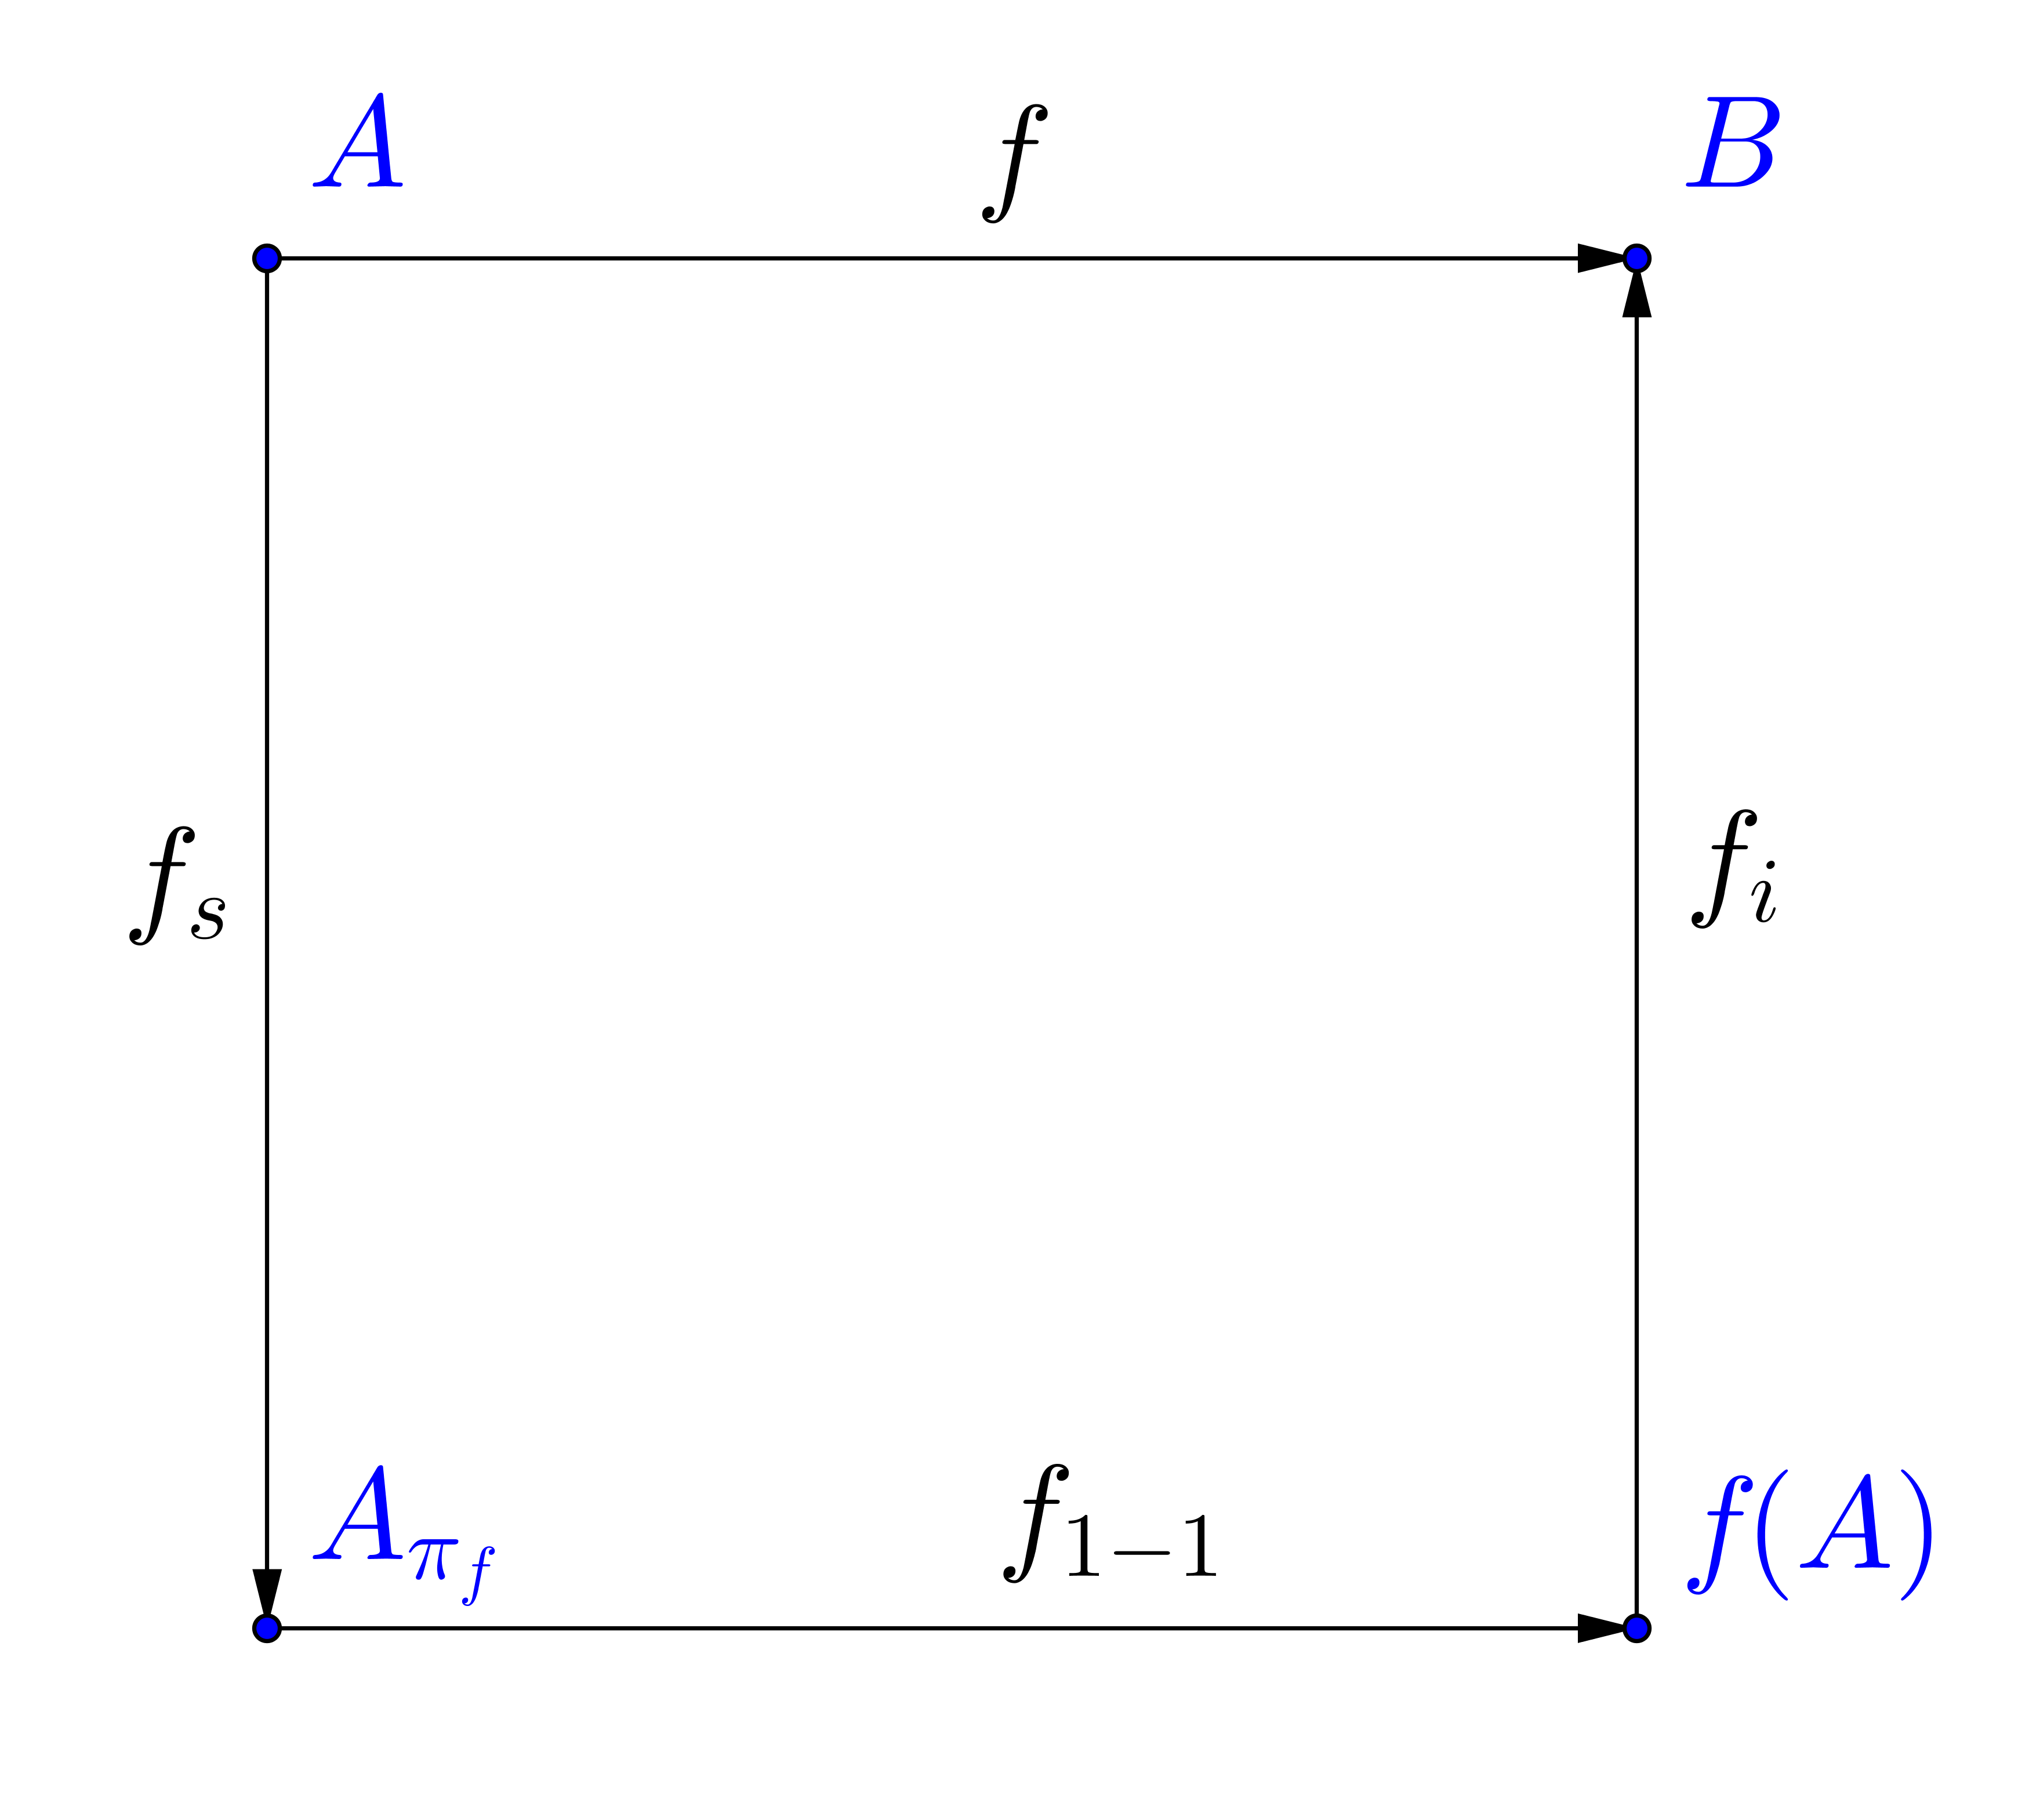
\includegraphics[width=0.6\linewidth]{lect2/InectBiectSuriect.png}
%\end{figure}

\begin{figure}[!h]
\begin{equation*}
\xymatrix{
A \ar[rr]^f\ar[dd]_{f_s} & & B\\
&\\
A_{\pi_f}\ar@{<->}[rr]^{f_{1-1}} & & f(A)\ar[uu]^{f_i}
}
\end{equation*}
\caption{Иллюстрация представления отображения $f$ как суперпозиции сюръекции, инъекции и биекции. $f_S$~--- сюръекция, $f_{1-1}$~--- биекция, $f_i$~--- инъекция}
\label{fig::superpos}
\end{figure}

На рис.~\ref{fig::superpos} изображены четыре множества: $A$, $B$, $A_{\pi_f}$~---фактор-множество по заданному отношению эквивалентности $\pi_f$, и $f(A)$~--- образ  $A$. Отображение $f_s$ сюръективно отображает множество $A$ в своё фактор-множество $A_{\pi_f}$ по следующему правилу: элементу множества $A$ ставится в соответствие класс эквивалентности, к которому он относится. Из-за ядерной эквивалентности отображения $f$, $A_{\pi_f}$ можно биективно отобразить в $f(A)$ с помощью отображения $f_{1-1}$. В свою очередь $f(A)$ инъективно вкладывается в $B$ как его подмножество с помощью тождественного преобразования $f_i$.

\section{О декартовом произведении множеств}
Поговорим о декартовом произведении множеств и о том, как его можно представить через другие операции с множествами. Итак, пусть есть множество индексов $\mathfrak{A} = \{\alpha\}$ и соответствующий этому множеству индексов набор множеств $\{A_{\alpha}|\ \alpha \in \mathfrak{A}\}$. Чему тогда равно произведение $\prod_{\alpha \in \mathfrak{A}}A_{\alpha}$? По крайней мере оно ненулевое, так как любое декартово произведение произвольного семейства непустых множеств в непустом количестве непусто (об этом свидетельствует аксиома выбора). Оказывается, что
\[
\prod_{\alpha \in \mathfrak{A}}A_{\alpha} = \{f|\ f:\ \mathfrak{A}\rightarrow\bigcup_{\alpha \in \mathfrak{A}}A_{\alpha}, \forall\alpha\in\mathfrak{A}: f(\alpha)\in A_{\alpha}\}
\]

Например, пусть
\[
A_{\alpha} = A_{(x, y)} = \{(x', y')| \rho((x,y), (x',y')) \leq 1\}
\]
Тогда
\[
\prod_{\alpha \in \mathfrak{A}}A_{\alpha} = \{f| f: R^2 \rightarrow R^2,\ \forall (x,y): \rho((x,y), f((x,y))) \leq 1\}
\]

\chapter{Лекция 3}
\section{Свободное произведение}
\textcolor{red}{Саня, Я вообще не уверен, что тут все правильно. Проверь меня, если сам понял хоть что-то в этой теме:). Надо ещё как то обосновать представление прямой суммы как специфического объединения. Я не понял почему оно так представляется. Очень может быть что я пропустил тут в определениях какое нибудь "для любого альфа", мне самому не совсем понятно}

\textcolor{blue}{Сева, это какая-то жесть!}

Прежде чем вводить свободное произведение, вспомним о понятии гомоморфизма, играющем важную роль в определении свободного произведения.

\begin{definition}
Пусть
$
\mathcal{R}^1 =
\begin{pmatrix}
A & r_1^1 & \ldots & r_k^1\\
  & n_1 & \ldots & n_k
\end{pmatrix}
$
и
$
\mathcal{R}^2 =
\begin{pmatrix}
B & r_1^2 & \ldots & r_k^2\\
  & n_1 & \ldots & n_k
\end{pmatrix}
$, отображение $f: A^m \rightarrow B$~--- гомоморфизм, если это отображение сохраняет все отношения, то есть пусть
\[
\forall l \in \{1, \ldots, k \} \; f(a_1^1, \ldots, a_1^m) = b_1, \ldots, f(a^1_l, \ldots, a_l^m) = b_l,
\]
тогда
\[
\forall t \in \{ 1,\ldots,m\} \; (a_1^t, \ldots, a_l^t) \in r_l^1 \Rightarrow (b_1, \ldots, b_l) \in r^2_l.
\]
\end{definition}

\begin{definition}[Свободное произведение]
Пусть имеется $\{A_{\alpha}|\ \alpha\in\mathfrak{A}\}$~--- некоторое множество алгебраических систем. Тогда алгебраическая система $B$, порождённая системами $A_{\alpha}$ так, что гомоморфизм $\varphi_{\alpha}: C \rightarrow A_{\alpha}$, где $C$~--- произвольная алгебраическая система, продолжается до гомоморфизма $f:\ C\rightarrow B$ называется свободным произведением и обозначается
\[
\mathop{\textstyle{\prod^*}}\limits_{\alpha\in\mathfrak{A}} A_{\alpha}.
\]
\end{definition}

%\begin{figure}[htbp]
%\centering
%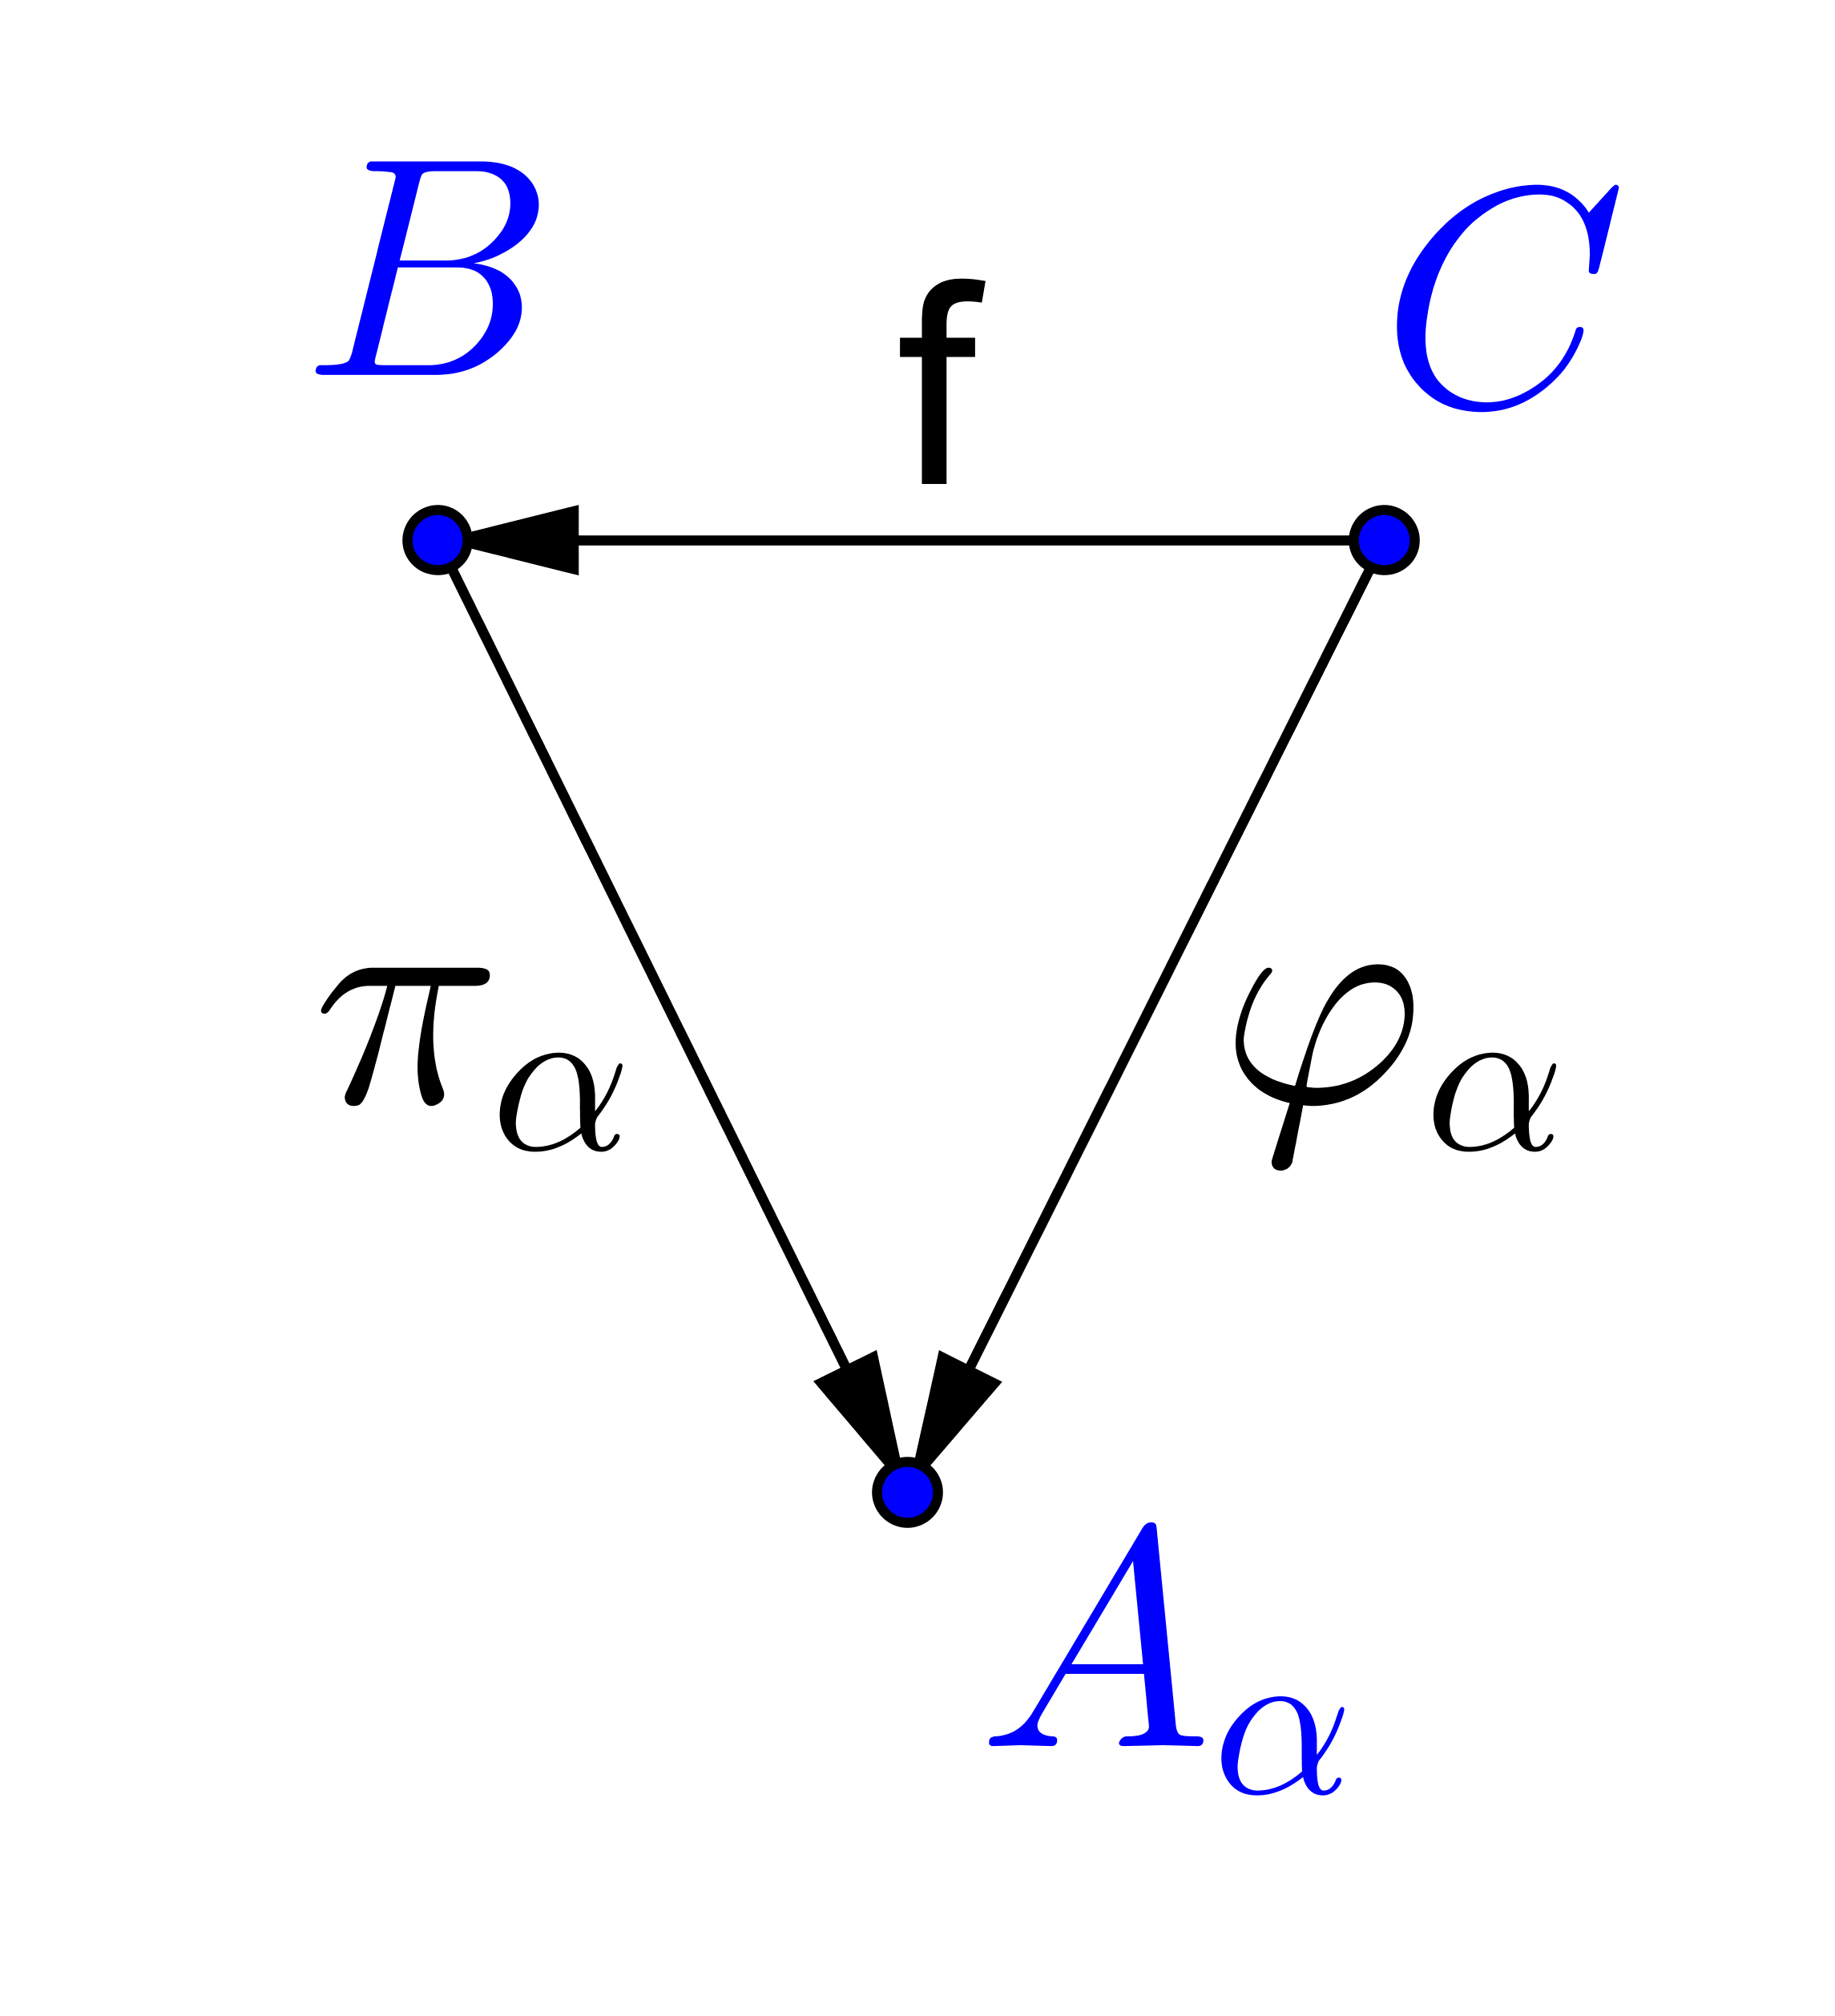
\includegraphics[width=0.3\linewidth]{lect3/FreeProduct.png}
%\end{figure}

На рисунке~\ref{fig::free_prod} видно, как работает это определение. Мы берём произвольное, но фиксированное $C$ и отображаем его всеми морфизмами $\varphi_{\alpha}$ во все $A_{\alpha}$. Тогда, имея морфизм $\pi_{\alpha}: B\rightarrow A_{\alpha}$ мы автоматически задаём единственный морфизм из $C$ в $B$. Важное замечание состоит в том, что, возможно, лектор ошибся, и перепутал свободное произведение с свободной суммой, которая будет определена в дальнейшем.

\begin{figure}[!h]
\begin{equation*}
\xymatrix{
B\ar[rd]_{\pi_{\alpha}} & & \ar[ll]_f C\ar[ld]^{\varphi_{\alpha}}\\
 & A_{\alpha} &
}
\end{equation*}
\caption{Иллюстрация к понятию свободного произведения}
\label{fig::free_prod}
\end{figure}

\section{Свободная сумма}
Данное понятие очень похоже по сути на понятие свободного произведения. Вы сами увидите, что конструкции практически идентичны.

\begin{definition}[Свободная сумма]
Пусть имеется $\{A_{\alpha}|\ \alpha\in\mathfrak{A}\}$~--- некоторое множество алгебраических систем. Тогда алгебраическая система $B$, порождённая системами $A_{\alpha}$, так, что гомоморфизм $g_{\alpha}: A_{\alpha} \rightarrow C$, где $C$~--- произвольная алгебраическая система, продолжается до гомоморфизма $g:\ B\rightarrow C$ называется свободной суммой и обозначается
\[
\mathop{\textstyle{\sum^*}}\limits_{\alpha\in\mathfrak{A}} A_{\alpha}.
\]
\end{definition}

%\begin{figure}[htbp]
%\centering
%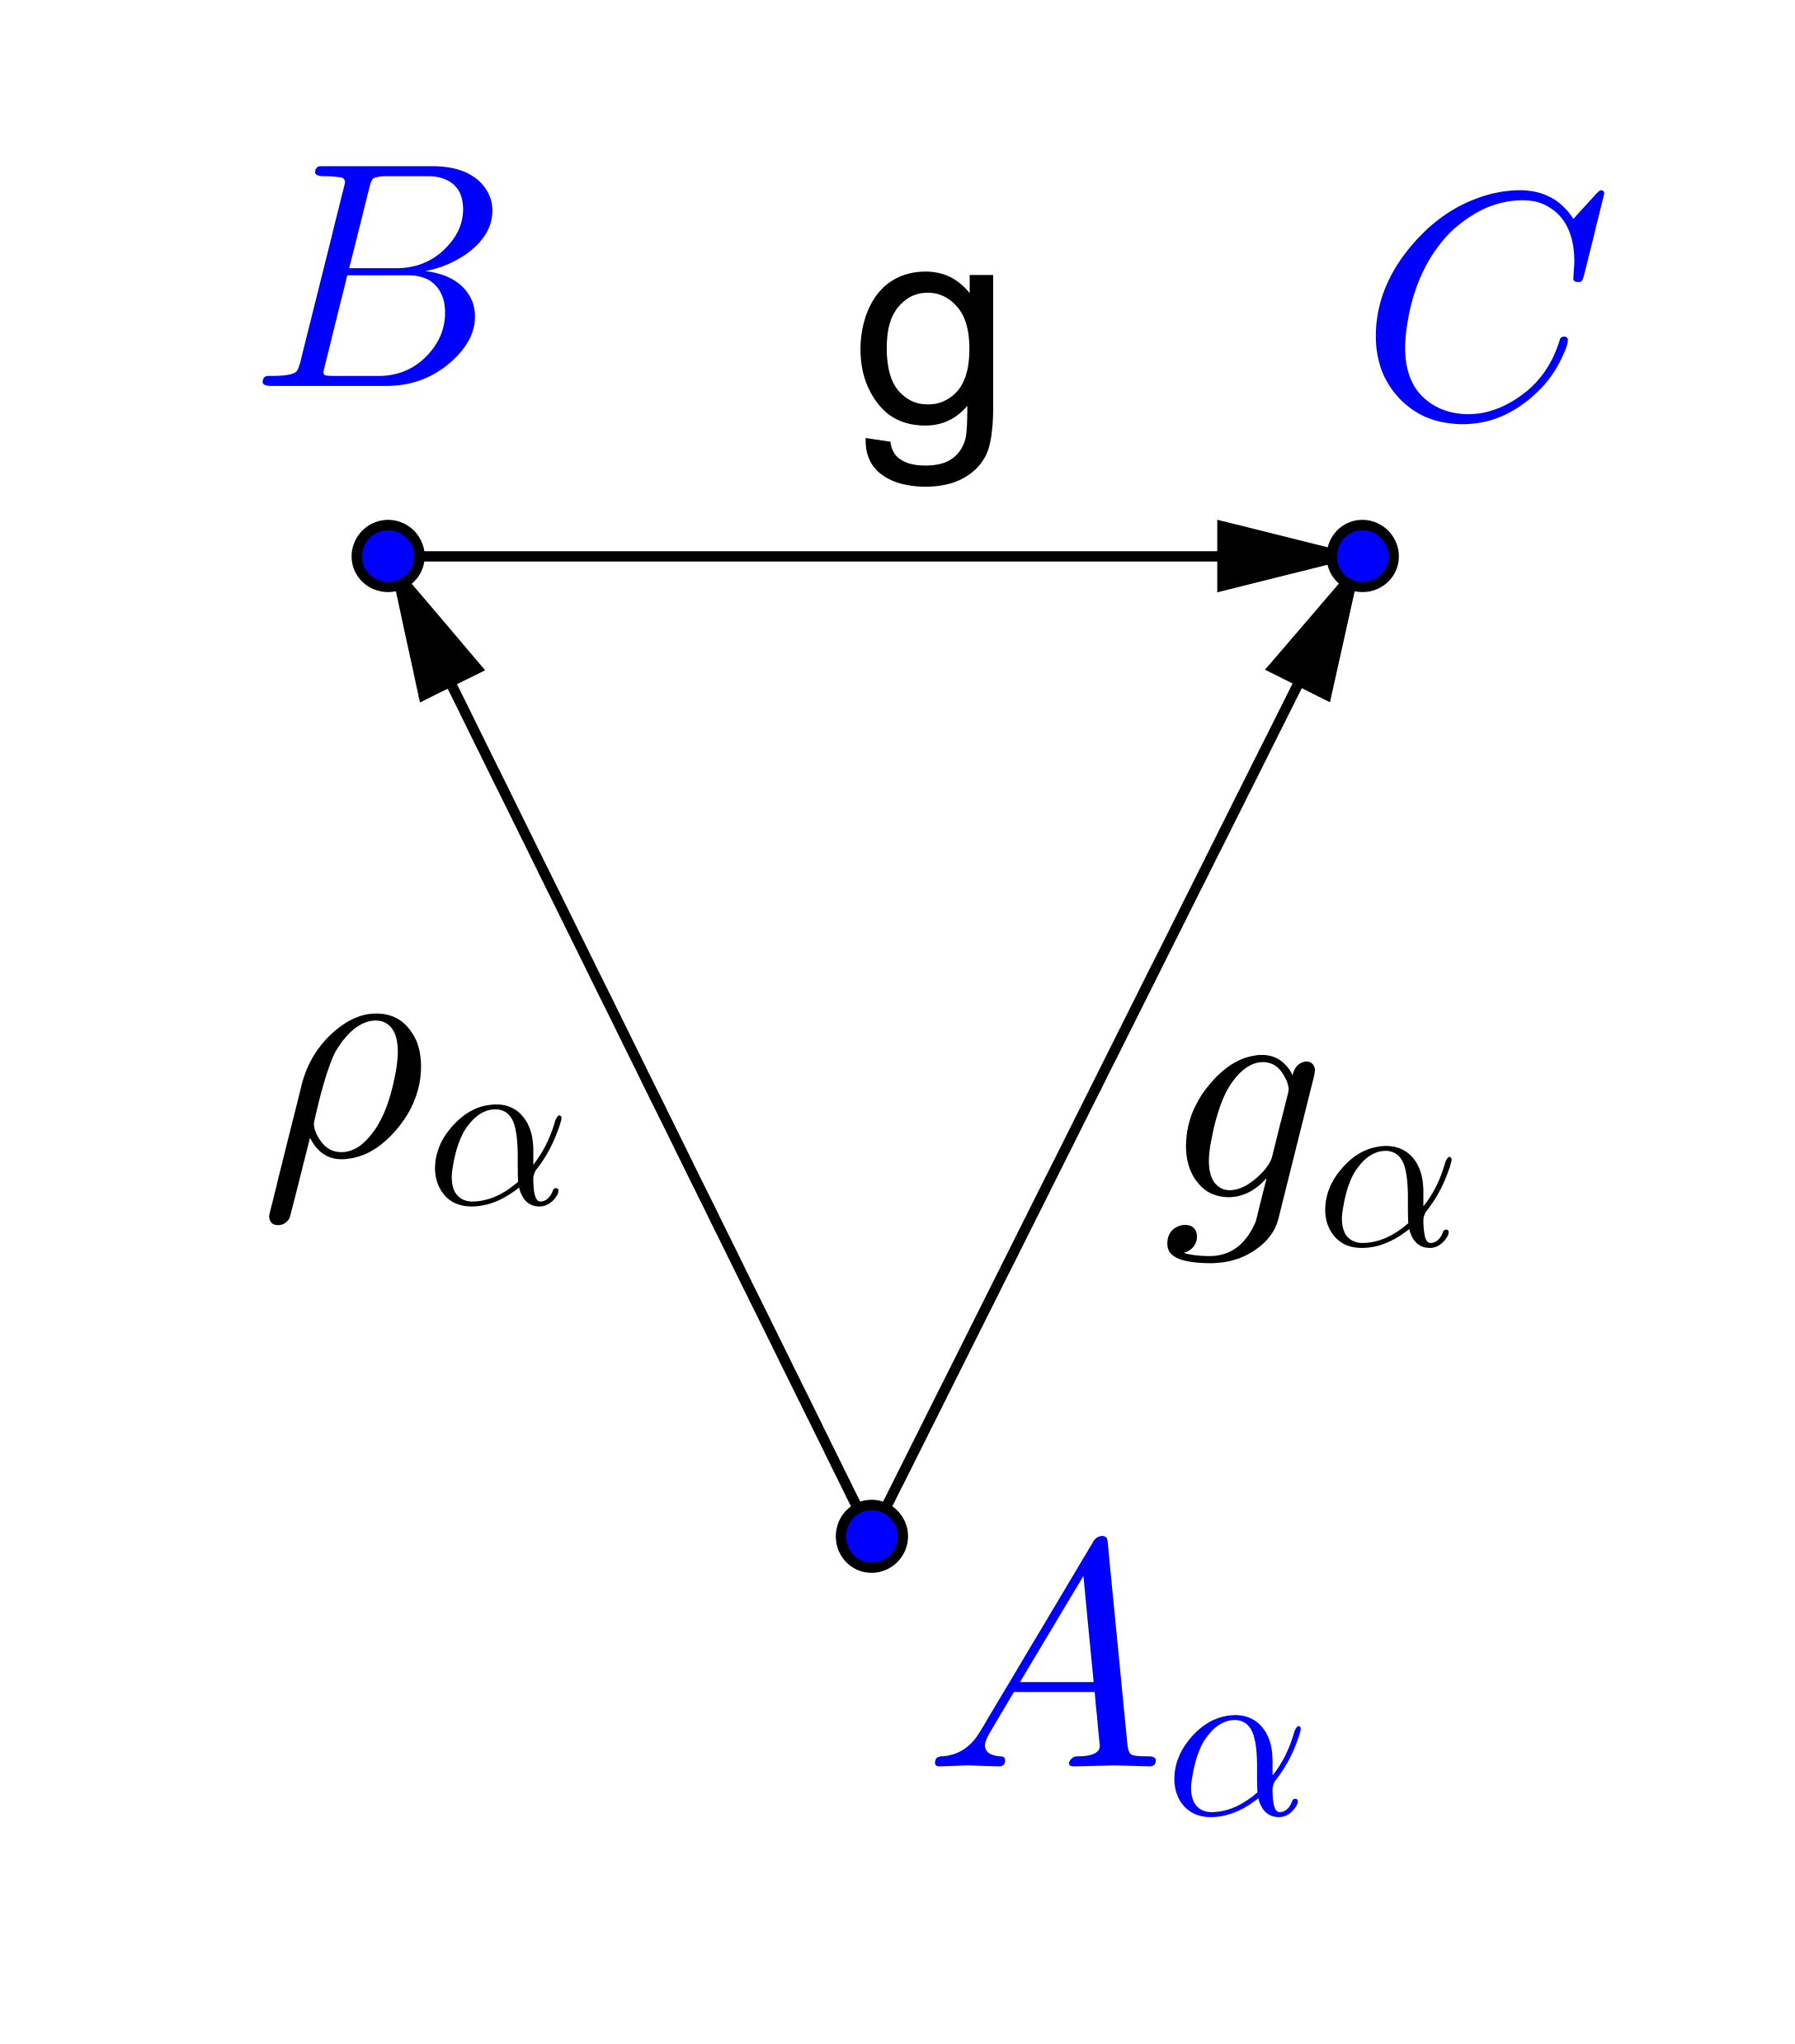
\includegraphics[width=0.3\linewidth]{lect3/FreeSum.png}
%\end{figure}

\begin{figure}[!h]
\begin{equation*}
\xymatrix{
B\ar[rr]^g & & C\\
 & A_{\alpha}\ar[lu]_{\rho_{\alpha}}\ar[ru]^{g_{\alpha}}
}
\end{equation*}
\caption{Иллюстрация к понятию свободной суммы}
\label{fig::free_sum}
\end{figure}

На рисунке~\ref{fig::free_sum} видно, как работает это определение. Его принцип очень схож с принципом свободного произведения. И на самом деле свободная сумма двойственна свободному произведению. На всякий случай напомним понятие двойственности из теории категорий:

\begin{definition}
Двойственность в теории категорий~--— соотношение между свойствами категории $C$ и так называемыми двойственными свойствами двойственной категории $C^*$. Взяв утверждение, касающееся категории $C$, и поменяв местами образ и прообраз каждого морфизма, так же как и порядок применения морфизмов, получим двойственное утверждение, касающееся категории $C^*$. Принцип двойственности состоит в том, что истинные утверждения после такой операции переходят в истинные, а ложные в ложные.
\end{definition}

Чем же является прямая сумма в более привычных терминах теории групп? На самом деле если множества $A_{\alpha}$ не пересекаются, то это просто объединение. Если же они пересекаются, то это объединение, которое ставит в соответствие $N = \sum_{\alpha\in\mathfrak{A}} |A_{\alpha}|$ элементное множество. Например, пусть $A^*_{\alpha} = \{(a, \alpha)\| a \in A_{\alpha}\}$. Тогда $B = \bigcup A^*_{\alpha}$.

\chapter{Лекция 4}
\section{Введение в категории}
\begin{definition}
Класс~--- это объект, который не может быть элементом множества или другого класса, в остальном свойства класса и множества совпадают.
\end{definition}

\begin{definition}
Будем обозначать $\Cql(\mathfrak{U})$ пространство всех матриц над произвольным неодноэлементным множеством $\mathfrak{U}$. Заметим, что если $\mathfrak{U}$ произвольные множества, то $\{\Cql(\mathfrak{U})\}$~--- это класс.
\end{definition}

Далее введём ключевое определение данного курса.

\begin{definition}[Категория]
Пусть $\Psi$ категория. Тогда
\begin{itemize}
  \item $Ob\Psi$~--- класс
  \item $\forall (A, B) \in Ob\Psi \rightarrow Hom_{\Psi} (A, B)$~--- множество. \\ То есть любой паре элементов из $Ob\Psi$ ставится в соответствие множество морфизмов из $A$ в $B$.
\end{itemize}
Таким образом, категория~--- это множество объектов и операций над ними.
\end{definition}

Рассмотрим свойства категории $\Psi$.
\begin{enumerate}
  \item Пусть есть 3 элемента $A, B, C \in \Psi$ и находятся в отношениях, изображённых на рис.~\ref{fig::property_1}.
\begin{figure}[!htbp]
%        \begin{center}
%            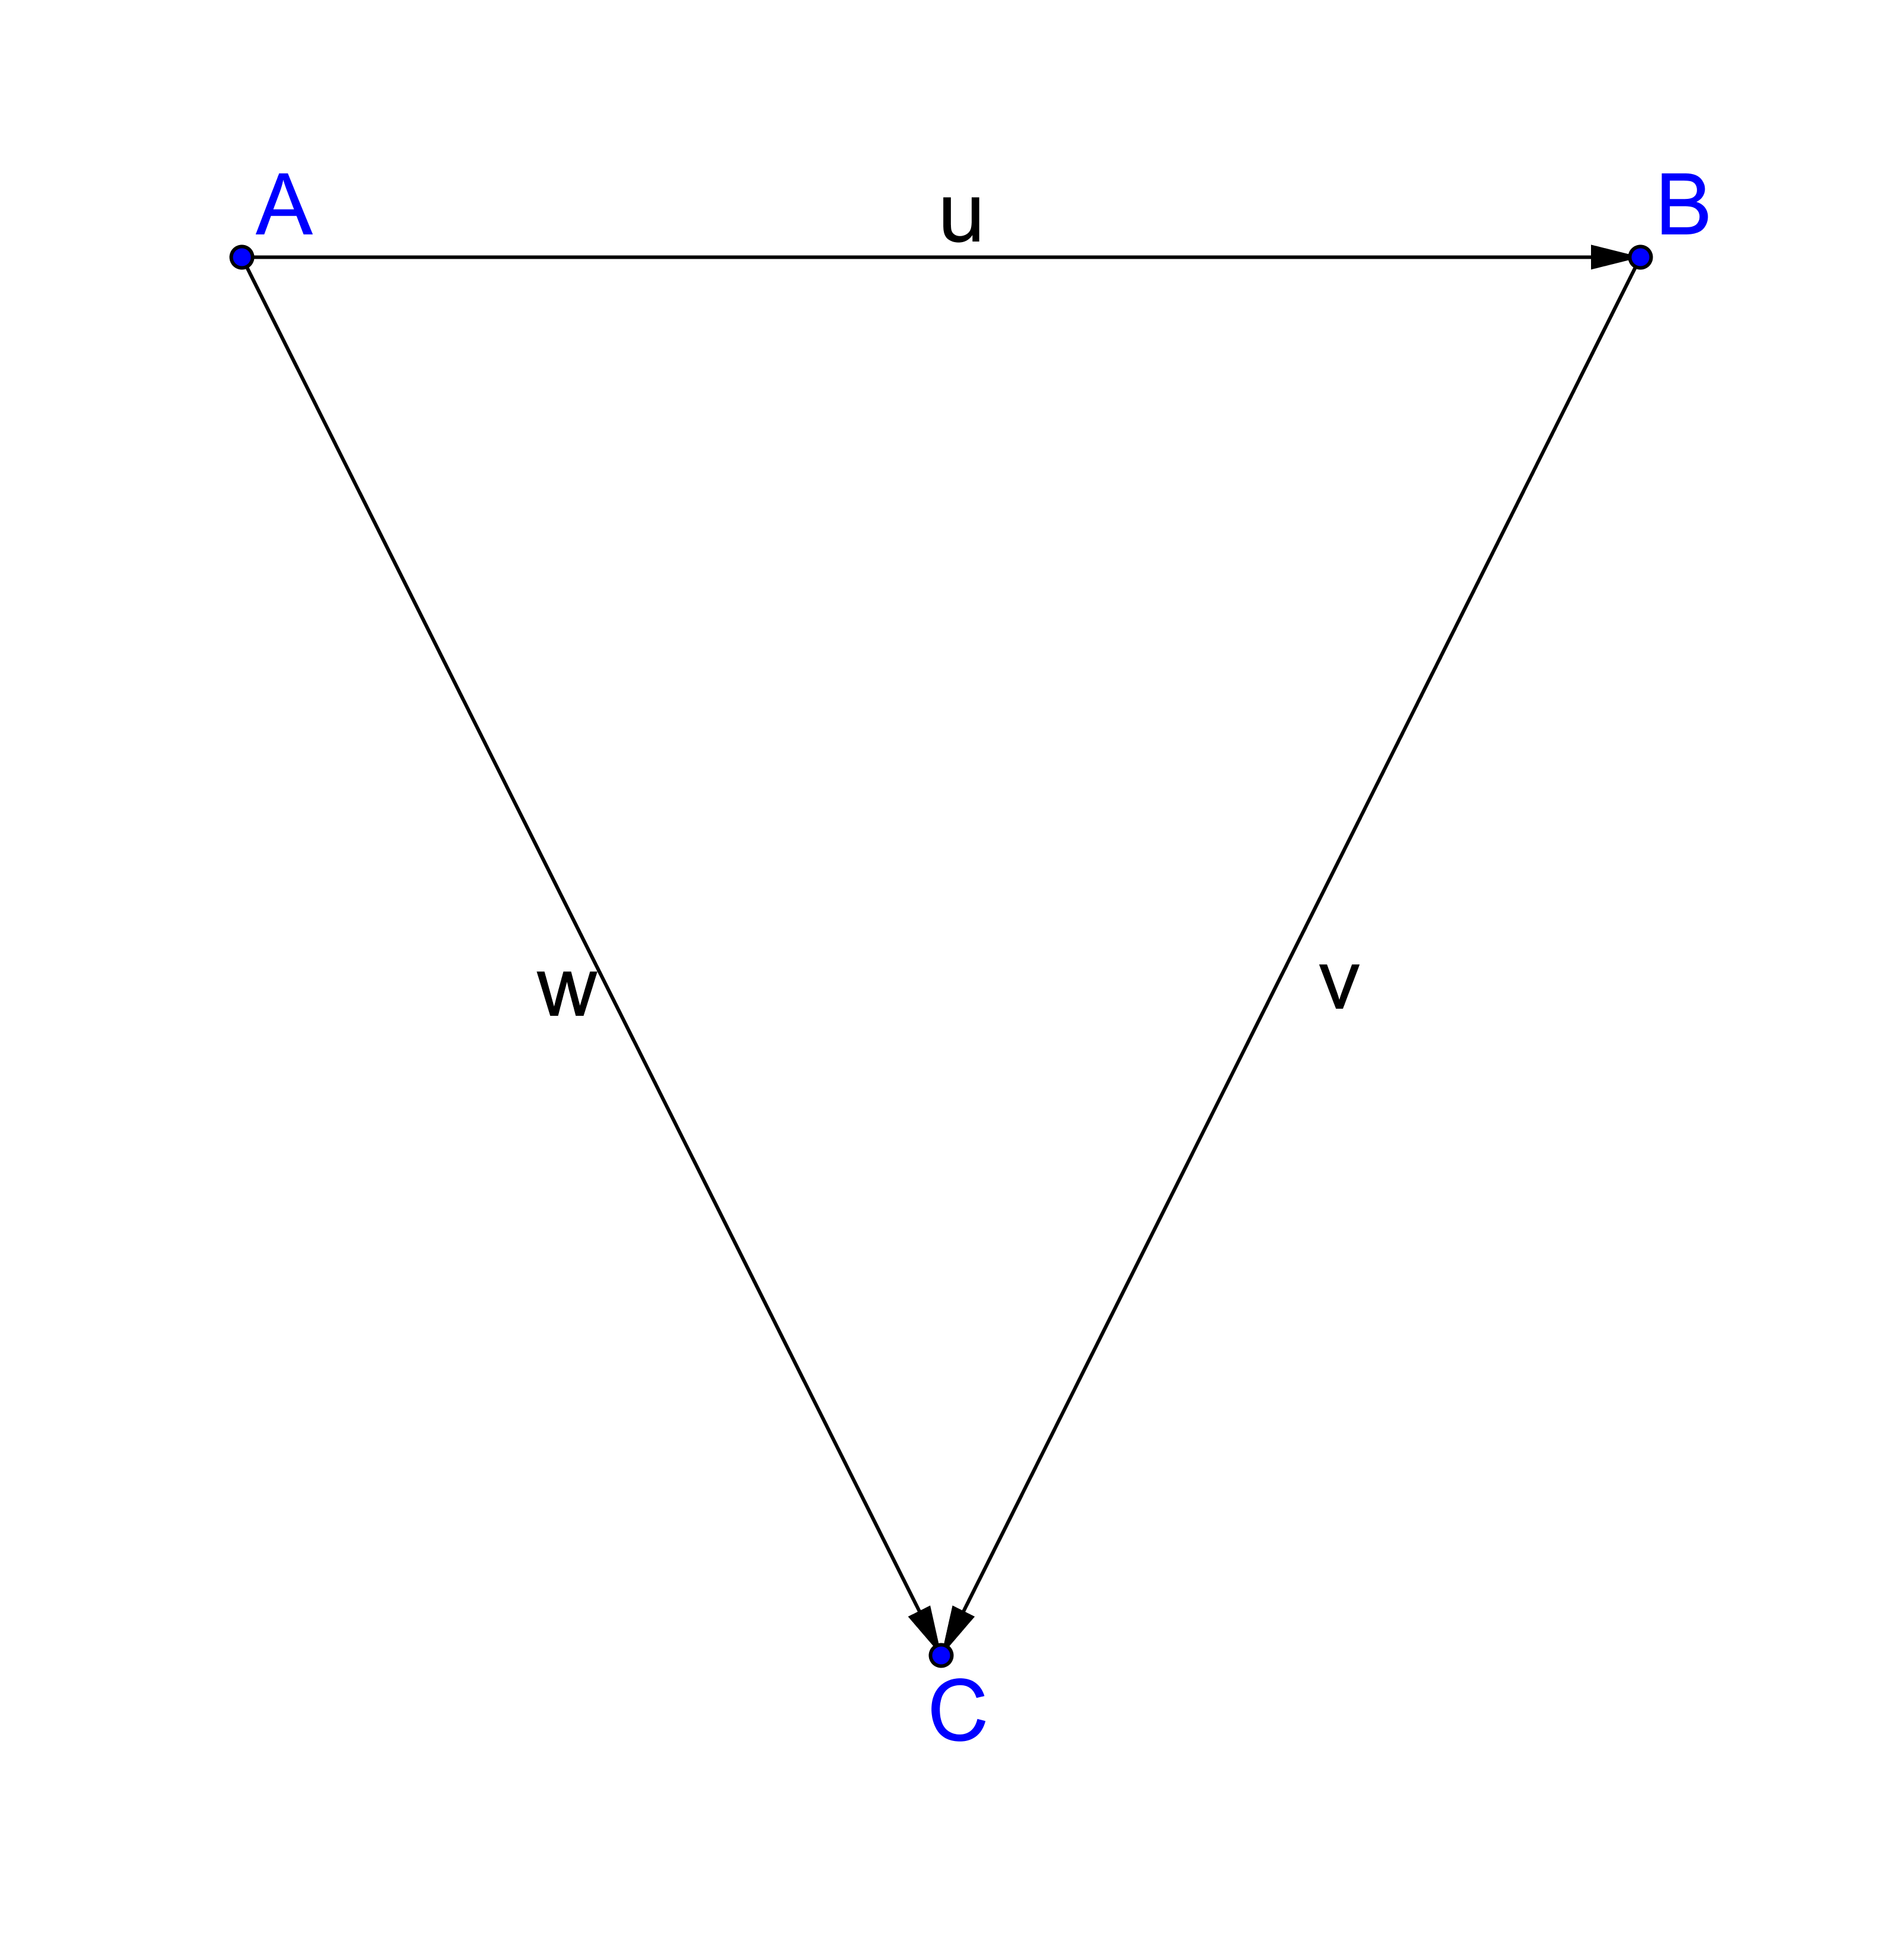
\includegraphics[width=0.3\linewidth]{lect5/Properity1pic1.png}
%        \end{center}
\begin{equation*}
\xymatrix{
A\ar[rr]^u\ar[rd]_w & & B\ar[ld]^v\\
 & C &
}
\end{equation*}
\caption{Отношения между объектами $A,B,C$.}
\label{fig::property_1}
\end{figure}

Тогда $w = v \circ u$. Таким образом определены суперпозиции для морфизмов. Более того, $(u \circ v) \circ w = u \circ (v \circ w)$ для любых $u, v, w$, для которых такая суперпозиция имеет смысл. А также существует единственный элемент $e_A$, такой что $u \circ e_A = u$ и $e_A \circ v = v$ (рис.~\ref{fig::identity}).
\begin{figure}[!htbp]
\begin{center}
\begin{minipage}[h]{0,45\linewidth}
%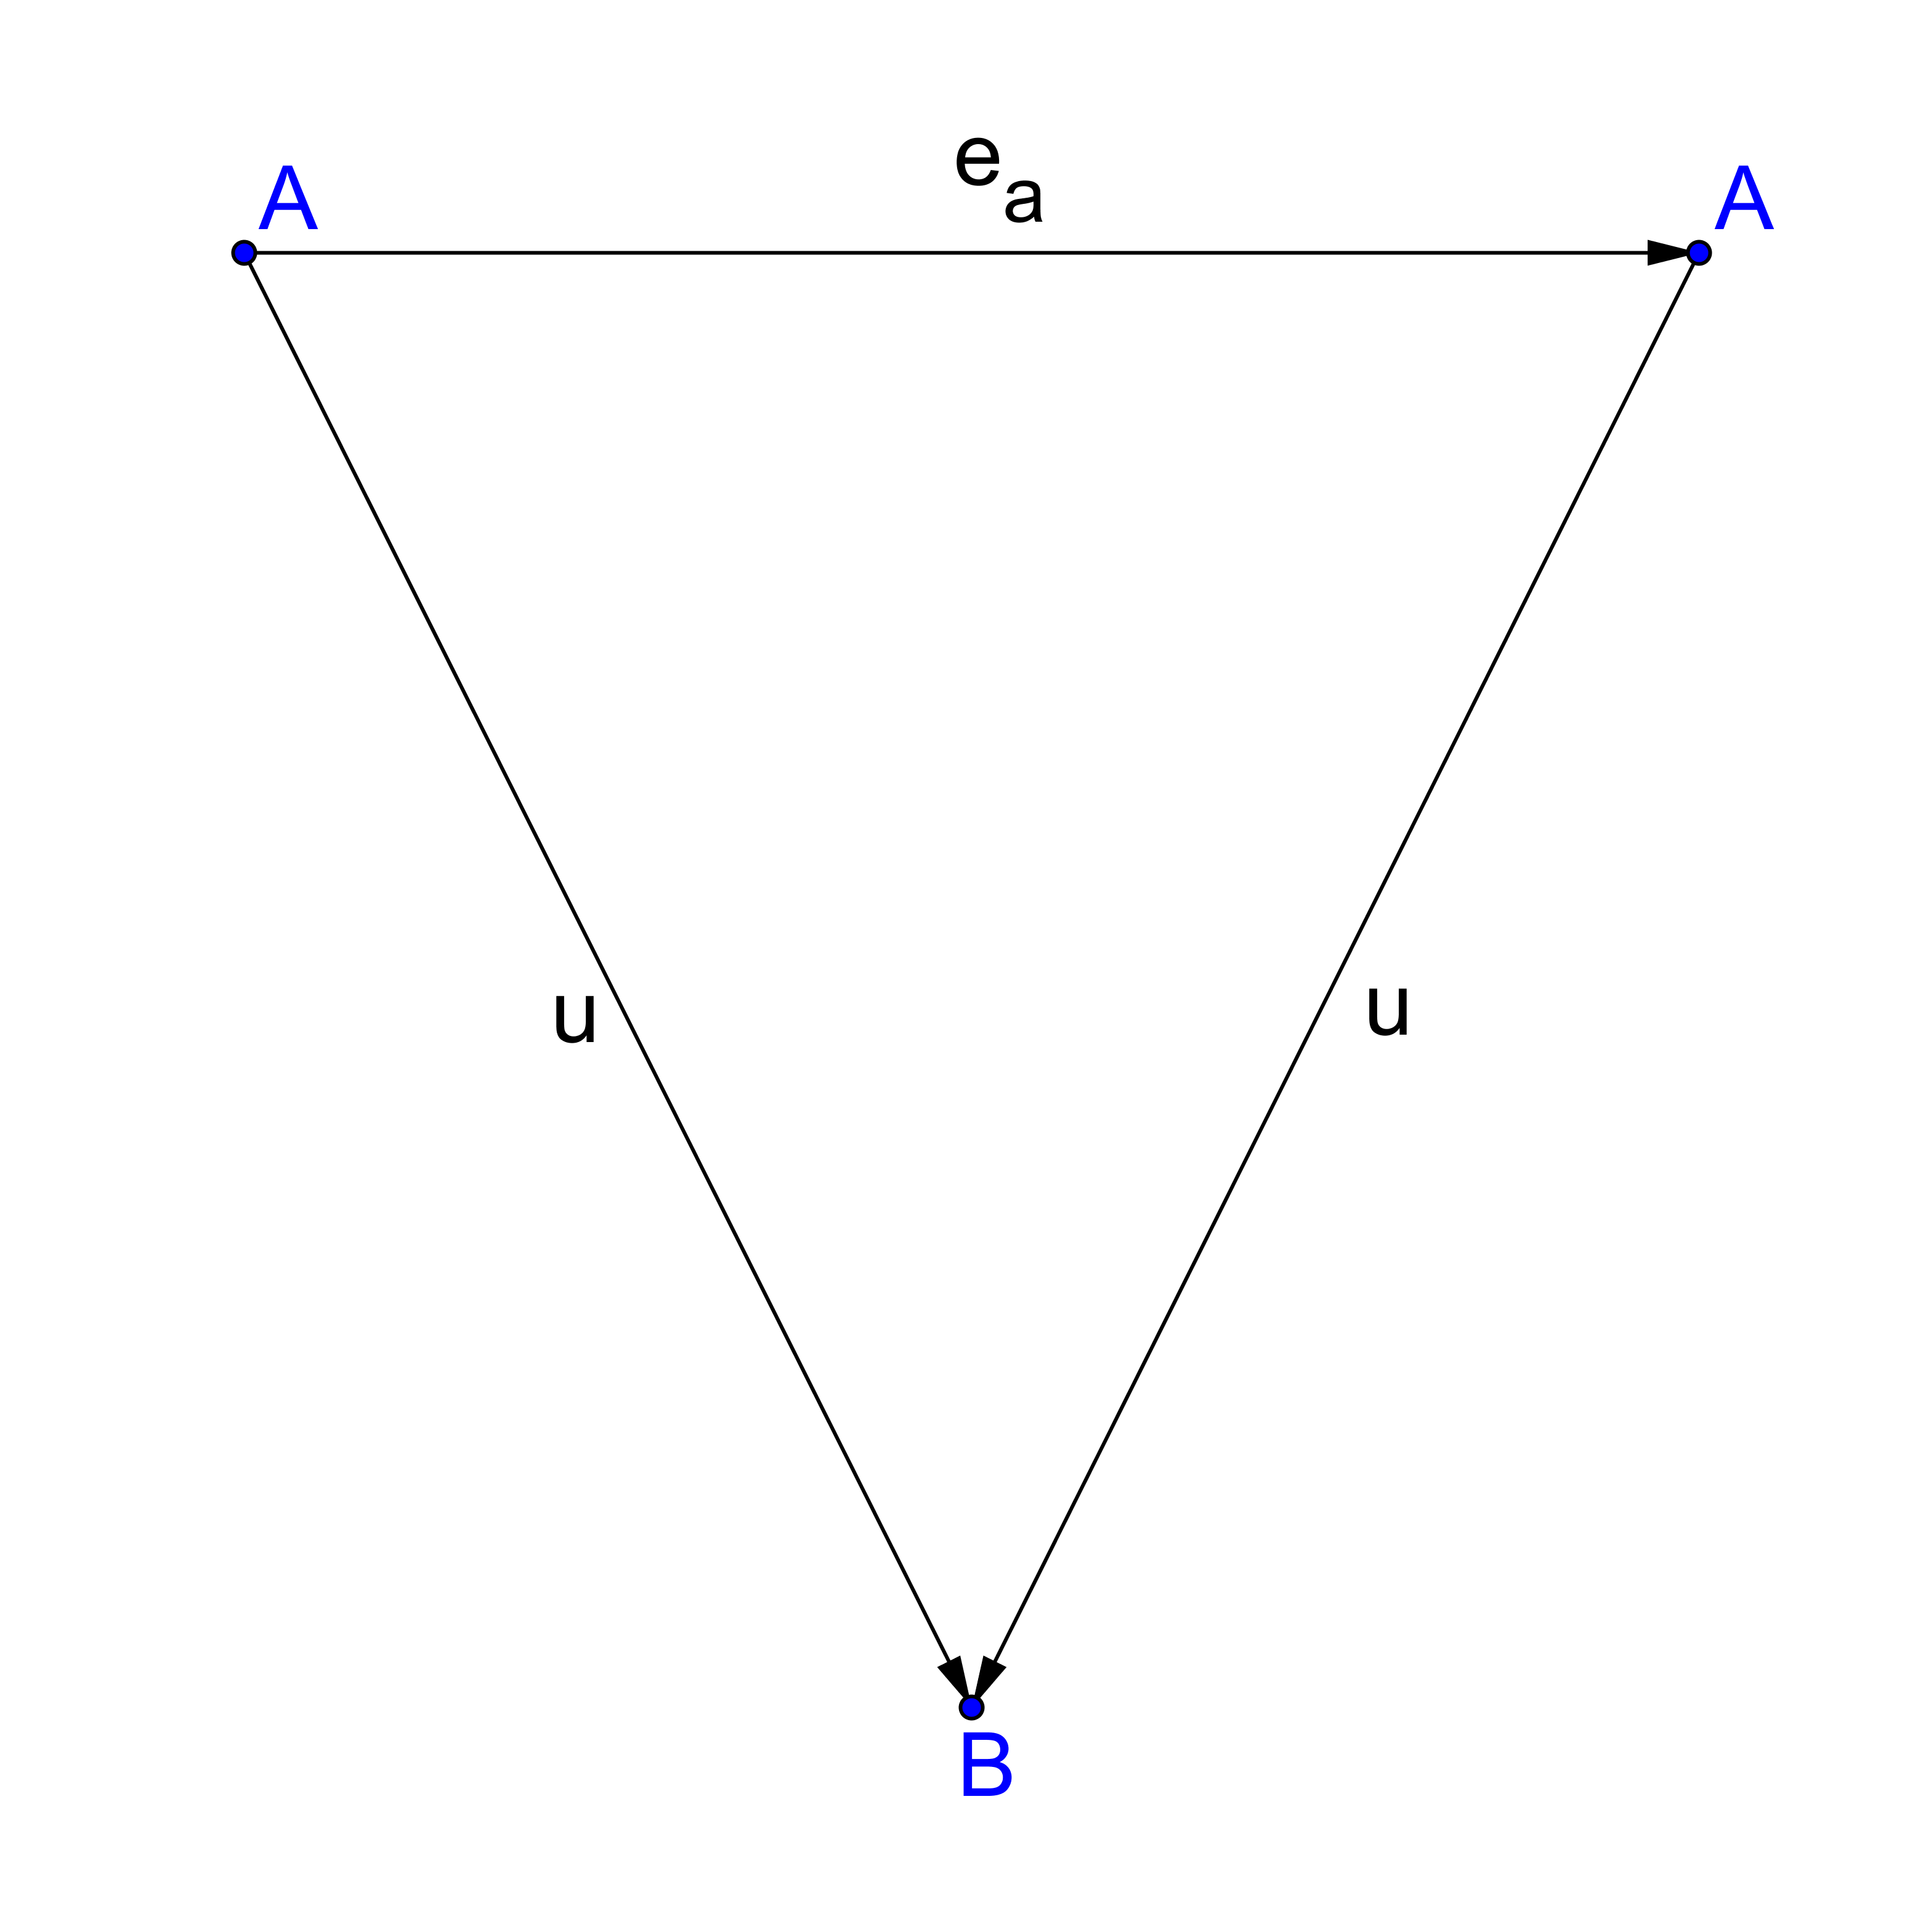
\includegraphics[width=1\linewidth]{lect5/Properity1pic2.png}
\begin{equation*}
\xymatrix{
A\ar[rr]^{e_A}\ar[rd]_u & & A\ar[ld]^u\\
 & B &
}
\end{equation*}
\end{minipage}
\begin{minipage}[h]{0.45\linewidth}
%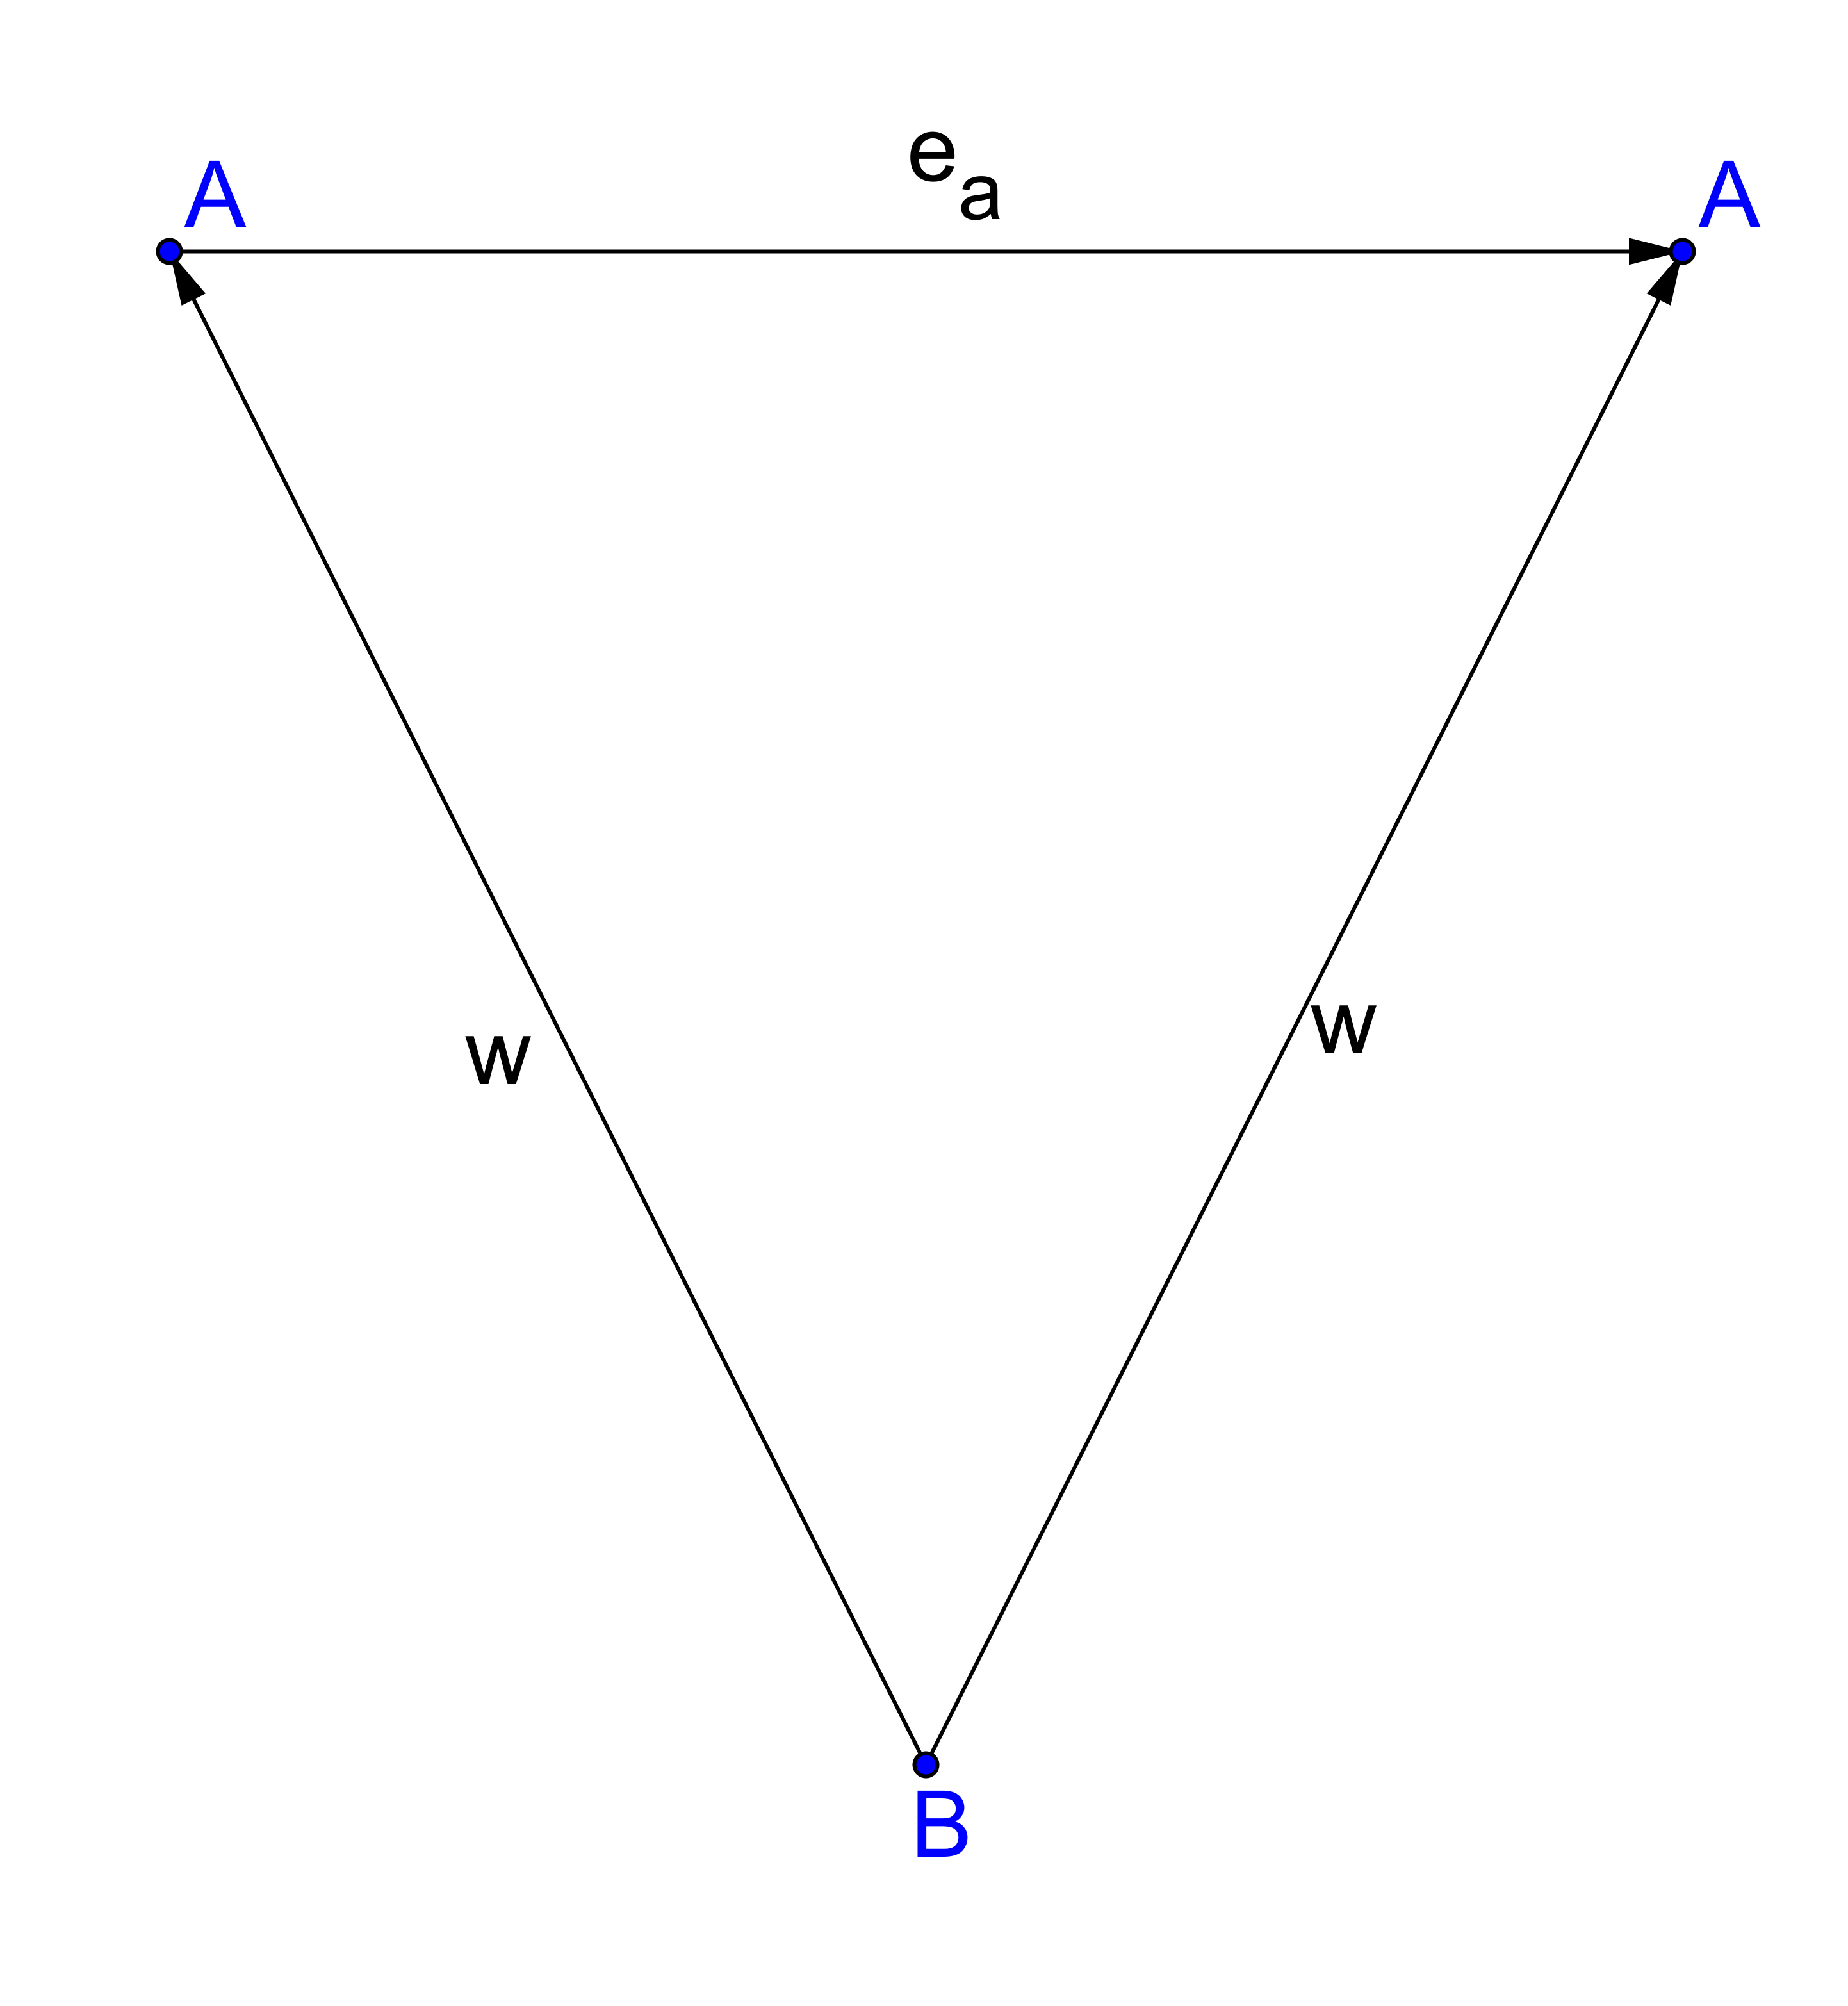
\includegraphics[width=1\linewidth]{lect5/Properity1pic3.png}
\begin{equation*}
\xymatrix{
A\ar[rr]^{e_A} & & A\\
 & B\ar[ru]_v\ar[lu]^v &
}
\end{equation*}
\end{minipage}
\end{center}
\caption{Свойства единичного элемента}
\label{fig::identity}
\end{figure}
\item $\Psi'$ подкатегория $\Psi$ если:
\begin{itemize}
\item $Ob\Psi'$~--- подкласс $Ob\Psi$
\item $\forall\ A, B \in Ob\Psi':\ Hom_{\Psi'} \subseteq Hom_{\Psi} (A, B)$
\end{itemize}
Причём, если во втором условии стоит равенство, то $\Psi'$~--- полная подкатегория категории $\Psi$.
\end{enumerate}

\begin{definition}
$\Psi$~--- полная категория, если при всех $A$ и  $B$: $ \bigcup\limits_p Hom_{\Psi}(A^p, B)(A) = B$.
\end{definition}

\paragraph{Пример категории.} Объекты~--- это множества $A, B$; морфизмы~--- это отображения из $2^A$ в $2^B$. Например, отображения из $\Cql(\mathfrak{U})$ в $\Cql(\mathfrak{V})$, коммутирующие со всеми перестановками строк.


\section{Дальнейшая формализация общей задачи}
Для начала введём несколько понятий, тут будут использоваться следующие обозначения: $ob = object,\ cl=class,\ i=initial,\ f=final$.
Приступим:
\begin{itemize}
  \item $\Upsilon=\{S\}$~--- множество объектов;
  \item $\mathfrak{D}_{ob}:\ \Upsilon\rightarrow\mathfrak{J}_{ob}$~--- отображение из множества объектов в множество информации об объектах;
  \item $K_1,\ldots,K_l;\ K_j \subseteq \Upsilon,\ j=\overline{1,l}$. Мы рассматриваем задачу классификации и $K_1,\ldots,K_l$~--- наши классы. Они являются элементами одного множества, но сами могут быть различны.
  \item $\mathfrak{D}_{cl}:\ 2^{\Upsilon}\rightarrow\mathfrak{J}_{cl}$
\end{itemize}
Наша задача:
\[
A:\ \mathfrak{J}_i \rightarrow \mathfrak{J}_f.
\]
Её решение может быть формализовано в различных вариантах:
\begin{enumerate}
  \item $\mathfrak{J}_i = \mathfrak{J}_{ob}\times\mathfrak{J}_{cl}$. В такой постановке мы игнорируем тот факт, что классов $l$.
  \item $\mathfrak{J}_i = \mathfrak{J}_{ob}\times\mathfrak{J}_{cl}^l$. Этот вариант лишён проблемы первого пункта и классы наши различны.
  \item $\mathfrak{J}_i = \mathfrak{J}_{ob}^q\times\mathfrak{J}_{cl}^l$. Ещё более сложный вариант, в котором участвует количество объектов $q$. Таким образом, $S_1,\ldots,S_q$~--- объекты, $(S_1,\ldots,S_q)\in\Upsilon^q$ и окончательно ($\mathfrak{D}_{ob}(S_1), \ldots, \mathfrak{D}_{ob}(S_q)) \in \mathfrak{J}_{ob}^q$. В такой постановке мы можем учесть зависимость объектов друг от друга.
  \item $\mathfrak{J}_i = \Cql(\mathfrak{J}),\ \mathfrak{J}_f = \Cql(\tilde{\mathfrak{J}})$, где $\Cql$~--- пространство $q\times l$ матриц над чем-либо. Данный вариант наиболее общий, и его мы будем в дальнейшем рассматривать, считая $\mathfrak{J},\ \tilde{\mathfrak{J}}$ неодноэлементными множествами (иначе множество матриц тривиально).
\end{enumerate}

Может показаться, что пункт 4 и 3 дают одинаковую задачу, но это не так. \textcolor{red}{Саня, Я не помню контрпример. Если у тебя есть - впиши}

\section{Задача Z и уточнение структуры структурной информации}
В новых терминах решение задачи Z формулируется таким образом. Пусть $\hat{I} \in \Cql(\mathfrak{J})$ и $\hat{\tilde{I}} \in \Cql(\tilde{\mathfrak{J}})$. Мы ищем такие алгоритмы $A$, что они являются допустимыми и $A(\hat{I}) = \hat{\tilde{I}}$

\begin{definition}
Алгоритм называется корректным на прецедентах, если $A(\hat{I}) = \hat{\tilde{I}}$
\end{definition}
\textcolor{red}{Саня, я тут не особо хорошо записывал. Проверь. Как то странновато вышло.}

До этого мы имели дело с множеством $\frakM^* = \{A| A(\frakI_i) = \frakI_f\}$. Теперь наши отображения действуют из $\hI$ в $\htI$, и нам уже недостаточно принадлежности $A$ к $\frakM^*$. Пусть $I_{str}^l$ такая, что $\frakM(I_{str}^l) = \{A| A(\hI) = A(\htI)\}$. Таким образом, $I_{str}^l$~--- часть структурной информации, отвечающая за то, что отображение действует из $\hI$ в $\htI$. Все же остальные ограничения на отображение $A$ обозначим $I_{str}^u$. Тогда $\frakM(I_{str}) = \frakM(I_{str}^l)\cap\frakM(I_{str}^u)$.

\section{Разбиение задачи на подзадачи}
Наша цель в данной секции разбить нашу исходную задачу на несколько подзадач. Идея данного разбиения изложена в диаграмме ниже:
\begin{equation*}
\xymatrix{
\Cql(\frakI)\ar[r]_A^\frakM\ar[d]_{\frakM^0}^B & \Cql(\tilde{\frakI})\\
\Cql(R)\ar[r]_{\mathfrak{F}}^F & \Cql(R)\ar[u]_C^{\frakM^1}
}
\end{equation*}
где $R$~--- неодноэлементное множество.

Будем называть $B$~--- распознающими операторами, $F$~--- корректирующими операторами, а $C$~--- решающим правилом, причём $F$ имеет арность $p$. Таким образом, $A = C\cdot F(B_1,\ldots, B_p)$, и, соответственно, $\frakM = \frakM^1\circ F(\frakM^0)$.

Обозначим $\Psi_{ql}$~--- такую категорию множеств, что $Ob\Psi_{ql} = \Cql(\frakU)$. Мы хотим рассматривать нашу задачу в некоторой подкатегории этой категории, но наложив на неё определённые ограничения.

Основная проблема состоит в том, что непонятно, как работать с $B_1,\ldots, B_p$ так, чтобы $F(B_1,\ldots, B_p): \Cql(\frakI)\rightarrow \Cql(R)$. Решением этой проблемы мы сейчас и займёмся.

Во-первых, введём понятия декартова произведения функций и диагонализации:
\begin{definition}
Пусть $f: A\rightarrow B$, $g: C\rightarrow D$. Тогда $(f\times g): A\times B\rightarrow C\times D$ и $(f\times g) (a, c) = (f(a), g(c)),\ a\in A, c\in C$.
\end{definition}
\begin{definition}
Пусть $f: A^n\rightarrow B$. Тогда $f_{\Delta}: A\rightarrow B$, и $f_{\Delta}(a) = f(a,\ldots, a)$~--- диагонализация функции $f$.
\end{definition}

Теперь рассмотрим следующую структуру.
Пусть
\[
\forall r=\{1,\ldots, s\}\ \forall k=\{1, \ldots, p_r \} \ B_k^r: \Cql(\frakI)\rightarrow\Cql(R);\ B_k^r\in\frakM^0,
\]
тогда
\[
B_1^r\times\ldots\times B_{p_r}^r: \Cql^{p_r}(\frakI)\rightarrow \Cql^{p_r}(R).
\]
Используя введённое выше определение диагонализации,
\[
(B_1^r\times\ldots\times B_{p_r}^r)_{\Delta}: \Cql(\frakI)\rightarrow \Cql^{p_r}(R).
\]
Также, введём $\forall r=\{1,\ldots, s\}\ F_r: \Cql^{p_r}(R) \rightarrow \Cql(R);\ F_r \in \mathfrak{F}$. Теперь определим
\[
B^{*r} = F_r\circ(B_1^r\times\ldots\times B_{p_r}^r)_{\Delta}: \Cql(\frakI)\rightarrow\Cql(R).
\]
И окончательно получили
\[
A = C\circ(B^{*1}\times\ldots\times B^{*r})_{\Delta}: \Cql(\frakI)\rightarrow \Cql(R).
\]
Отсюда вытекает определение:
\begin{definition}
$\Psi$~--- допустимая подкатегория $\Psi_{ql}$, если она замкнута относительно диагонализации и произведения отображений.
\end{definition}


\chapter{Лекция 5}
\section{Определение инъекции и сюръекции через морфизмы}

Рассмотрим множества $A, B, C$ и $D$ и отображения $g_1, g_2$, $u$ и $h_1, h_2$:
\begin{equation*}
\xymatrix{
C\ar@/^/[r]^{g_1}\ar@/_/[r]_{g_2} & A\ar[r]^u & B\ar@/^/[r]^{h_1}\ar@/_/[r]_{h_2} & D
}
\end{equation*}

\begin{definition}[Мономорфизм]
Отображение $u:\ A \rightarrow B$ называется мономорфизмом iff при любых $C$, $g_1$ и $g_2$, таких что $g_1:\ C \rightarrow A$, $g_2:\ C \rightarrow A$ и $g_1 \neq g_2$ выполнено $u \circ g_1 \neq u \circ g_2$ в смысле равенства элементов множества морфизмов.
\end{definition}

Мономорфизм~--- это обобщение инъективного отображения.
\begin{definition}[Эпиморфизм]
Отображение $u: A \rightarrow B$ называется эпиморфизмом iff $\forall D$ и $\forall$ $h_1: B \rightarrow D$ и $h_2: B \rightarrow D$, таких что $h_1 \neq h_2$ выполнено $h_1 \circ u \neq h_2 \circ u$.
\end{definition}

Эпиморфизм~--- обобщение сюръективного отображения.

\begin{definition}
Отображение $u: A \rightarrow B$~--- биекция или биморфизм, если одновременно мономорфизм и эпиморфизм.
\end{definition}

\begin{definition}
Отображение $u: A \rightarrow B$~--- изоморфизм, если $\exists u^{-1}: B \rightarrow A$ такое что $u^{-1} u = e_A$ и $u u^{-1} = e_B$:
\begin{equation*}
\xymatrix{
A\ar[rr]^u & & B\ar[ld]^{u^{-1}}\\
 & A\ar[lu]^{e_A} &
}
\end{equation*}
\end{definition}

В категории множеств каждый биморфизм является изоморфизмом, но в общем случае свойство <<быть изоморфизмом>> сильнее свойства <<быть биморфизмом>>, то есть любой изоморфизм есть биморфизм, но не любой биморфизм есть изоморфизм..

Пример категории, для которой биморфизм не есть изоморфизм:

\chapter{Лекция 6}
\section{Переход к категориям}
Для начала введем несколько упрощающих запись обозначений:
\begin{itemize}
  \item $Hom_{\Psi}(\Cql(\frakU),\ \Cql(\frakW)) = H(\frakU,\ \frakW)$
  \item $\bigcup_{p=0}^{\infty}Hom_{\Psi}(\Cql^p(\frakU),\ \Cql(\frakW)) = \calH(\frakU,\ \frakW)$
\end{itemize}
\textcolor{red}{Саня, Я не нашёл нужную букву под фигурное W. Пока что там стоит mathfrak{W}}
\begin{definition}
Категория $\Psi$ называется полной категорией, если при любых неодноэлементных $\frakU$ и $\frakV$ выполнено
\[
\calH(\frakU, \frakV)(\Cql(\frakU)) = \Cql(\frakV).
\]
\end{definition}

Определим также понятие регулярной задачи. Пусть у нас есть множество $\mathfrak{Z}=\{Z\}$~--- множество задач Z. Регулярность можно определять несколькими способами, например:
\begin{definition}[Регулярность по Журавлеву]
Задача регулярна, если разрешима для любой $\htI$.
\end{definition}
\begin{definition}
Задача называется регулярной, если существует окрестность $O(Z)\subseteq \mathfrak{Z},\ Z\in O(Z)$ такая, $\forall Z_i\in O(Z) \rightarrow Z_i$~--- разрешима.
\end{definition}
Мы будем пользоваться вторым определением.
Таким образом, каждой задаче $Z$ задан в соответствие набор $((\hI,\ \htI), I_{str}^u)$, $O(Z) = \{Z'| Z' \leftrightarrow ((\hI,\ \htI'), I_{str}^u)\}$. Теперь будем работать не с $I^u_{str}$, а с категорией $\Psi$~--- допустимой категорией $\Psi_{ql}$.

\textcolor{red}{Саня, итак, получилось уберкоротко и нихрена не понятно (частично понятно, но последняя строчка вообще хрен знает откуда вылезла) Плюс я картинку не рисовал (квадрат со стрелочками). Надо с обозначениями для них разобраться.}

\chapter{Лекция 7}
\section{Понятие базы и формализация требований к морфизмам}
Нам потребуется понятие базы для последующих исследований. Введём его схожим с линейными пространствами способом.
\begin{definition}
Множество $X\subseteq \Cql(\frakU)$ называется базой в $\Psi$, если $\calH(\frakU,\frakU)(X)\ =\ \{\hfrakU| \hfrakU \in \Cql(\frakU),\ \exists p\ \exists u\ \exists (\hfrakU^1,\ldots,\hfrakU^p) \in X^p: \hfrakU = u(\hfrakU^1,\ldots,\hfrakU^p)\}$.

Данная развёрнутая запись является обобщением простой идеи:  $\calH(\frakU,\frakU)(X) = \Cql(\frakU)$.

Или ещё проще~--- из множества $X$ с помощью всех морфизмов из $\Psi $можно получить любую матрицу из $\Cql(\frakU)$.
\end{definition}
Однако, этого определения нам недостаточно, так как в нашей задаче мы смотрим морфизмы из одного множества в другое. Поэтому нам нужно множество $X$ в первом множестве, являющееся базой во втором. Это приводит нас к следующему определению.
\begin{definition}
Множество $X\subseteq \Cql(\frakU)$ называется базой в $\Cql(\frakU)$ для $\Cql(\frakW)$, если $\calH(\frakU,\frakW)(X) = \Cql(\frakW)$.
\end{definition}
Также для доказательства теоремы нам потребуется понятие полной категории.
\begin{definition}
$\Psi$~--- полная категория, если при всех $\frakU$ и  $\frakW$: $\calH(\frakU,\frakW)(\Cql(\frakU)) = \Cql(\frakW)$. Иначе, если $\Cql(\frakU)$ база в $\Cql(\frakU)$ для $\Cql(\frakW)$.
\end{definition}

Всё это приводит нас к следующей теореме.
\begin{theorem}
Пусть $\Psi$~--- полная допустимая категория, $\frakU,\ \frakW$~--- множества. Тогда
\[
(X \; \text{--- база})\Leftrightarrow(X \; \text{--- база в} \; \Cql(\frakU) \; \text{для} \; \Cql(\frakW)).
\]
\end{theorem}
\begin{proof}
\textbf{Необходимость.} Пусть $X$~--- база. Возьмём $\hat{V} \in \Cql(\frakW)$ и покажем, что мы можем получить его из элементов $X$ с помощью морфизмов из $\Psi$.

Так как $\Psi$~--- полна $\Rightarrow \exists p \in \mathbb{N} \ \exists u \in Hom_{\Psi}(\Cql^p(\frakU), \Cql(\frakW))\ \exists \hu^1,\ldots,\hu^p \in \Cql^p(\frakU):\ \hat{V} = u(\hu^1,\ldots,\hu^p)$.
И $\forall k\in\{1,\ldots,p\}\ \exists u_k \in \calH(\frakU, \frakU)\ \exists \hu'^1_k,\ldots,\hu'^{n_k}_k \in X^{n_k}:\ \hu^k = u_k(\hu'^1_k,\ldots,\hu'^{n_k}_k)$.

Подставим в выражение $\hat{V} = u(\hu^1,\ldots,\hu^p)$ выражения для $\hu^i$. Таким образом, получим:
\[
\hat{V} = u(u_1(\hu'^1_1,\ldots,\hu'^{n_1}_1),\ldots,u_p(\hu'^1_p,\ldots,\hu'^{n_p}_p)) = u\circ(u_1\times\ldots\times u_p)(\hu'^1_1,\ldots,\hu'^{n_p}_p).
\]
Ввиду допустимости категории $\Psi$, морфизм $u\circ(u_1\times\ldots\times u_p) \in \Psi$ и мы получили с помощью морфизмов $\Psi$ любой элемент из $\Cql(\frakW)$.

\textbf{Достаточность.} Пусть $X$~--- база в $\Cql(\frakU)$ для $\Cql(\frakW))$. Доказательство достаточности аналогично доказательству необходимости.

Возьмём $\hat{U} \in \Cql(\frakU)$. Поскольку $\Psi$~--- полна, то $\hat{U} = u(\hv^1,\ldots,\hv^p)$ и $\hv^k = v_k(\hv'^1_k,\ldots,\hv'^{n_k}_k)$, причём все $\hv'^i_j \in X$.\\
Таким образом, $\hat{U} = u(v_k(\hv'^1_1,\ldots,\hv'^{n_1}_1),\ldots,v_k(\hv'^1_p,\ldots,\hv'^{n_p}_p)) = v\circ(v_1\times\ldots\times v_p)(\hv'^1_1,\ldots,\hv'^{n_p}_p)$.\\
Ввиду допустимости категории $\Psi$, морфизм $v\circ(v_1\times\ldots\times v_p) \in \Psi$ и мы получили с помощью морфизмов $\Psi$ любой элемент из $\Cql(\frakU)$.
\end{proof}

Рассмотрим теперь несколько условий, необходимых и достаточных, чтобы $X$ была базой.
\begin{itemize}
  \item $\calH(\frakW, \frakV)(X) = \Cql(\frakV)$ iff $X$~--- база в $\Cql(\frakW)$.
  \item $\calH(\frakW, \frakV)\calH(\frakW, \frakW)(X) = \Cql(\frakV)$ iff $X$~--- база.
  \item $\calH(\frakW, \frakV)\calH(\frakW, \frakW)H(\frakV, \frakW)(X)=\Cql(\frakV)$. Это необходимо, чтобы $X$ было базой, но может быть не достаточно. Проблема в $H(\frakW, \frakV)$~--- слишком бедное множество морфизмов.
  \item $H(\frakW, \frakV)(X) = \Cql(\frakV)$ - аналогично, это необходимо, чтобы $X$ было базой.
\end{itemize}
Последние два свойства оказались необходимыми, но не достаточными. Оказывается, что справедлива теорема:

\begin{theorem}
Если $X$ - одноэлементная база(то есть $|X|=1$), тогда в свойствах 3 и 4 достаточно, чтобы $X$ было базой.
\end{theorem}
\begin{proof}
В обоих свойствах нужно "преодолеть" $H(\frakW, \frakV)$. Рассмотрим любой элемент $V\in\frakV$. Так как $X$ - база, то $V=u(\hu^1,\ldots,\hu^p)$, причём $(\hu^1,\ldots,\hu^p)\in X^p$. Но $X$ - одноэлементная база, а значит все $\hu^i$ равны некоторому $\hu^0$ и окончательно $V = u(\hu^0,\ldots,\hu^0) = u_{\Delta}(\hu^0) \in H(\frakW, \frakV)$. Таким образом для одноэлементной базы достаточно и такого бедного множества морфизмов как $H(\frakW, \frakV)$, чтобы получить всё множество $\frakV$.
\end{proof}

\section{Уточнения требований накладываемых на морфизмы разбиения}
В этом разделе все обозначения соответствуют обозначениям на следующей диаграмме:
\begin{equation*}
\xymatrix{
\Cql(\frakU)\ar[r]^\frakM\ar[d]_{\frakM^0 \subseteq \calH(..)} & \Cql(\frakV)\\
\Cql(\frakW)\ar[r]_{\mathfrak{F}} & \Cql(\frakW)\ar[u]_{\frakM^1 \subseteq \calH(..)}
}
\end{equation*}
Из данной диаграммы видно, что $\frakM = \frakM^1\circ\mathfrak{F}\circ\frakM^0$.\\

Для начала приведём общий критерий регулярности задач классификации:
\begin{theorem}
Задача $Z$~--- регулярна iff $\{\hI\}$ - база $\Psi$.
\end{theorem}
А также, несколько новых определений:
\begin{definition}
$\frakM$~--- полно, если в $\frakM$ разрешима любая регулярная задача $Z\leftrightarrow(\Psi,\hI,\htI)$.
\end{definition}
\begin{definition}
$\frakM^0 \subseteq H(\frakV, \frakW)$ называется 1~-~$\Gamma$~-полным, если для любой одноэлементной базы $X$ выполнено $\frakM^0(X) = \Cql(\frakW)$.
\end{definition}
Оказывается, справедлива следующая теорема:
\begin{theorem}
$\frakM$~--- полно iff $\frakM$~--- 1~-~$\Gamma$~-полно.
\end{theorem}
Введём ещё несколько понятий, потребующихся нам в будущем.
\begin{definition}
$\frakM^0\subseteq H(\frakV, \frakW)$~--- полная модель алгебраических операторов, если $\exists \mathfrak{F}, \frakM^1: \frakM = \frakM^1\circ\mathfrak{F}\circ\frakM^0$~- полно.
\end{definition}
\begin{definition}
$\frakM^0\subseteq H(\frakV, \frakW)$ называется слабо 1~-~$\Gamma$~-полным, если для любой одноэлементной базы $X\subseteq\Cql(\frakV)$ выполнено $\frakM^0(X)$~--- база в $\Cql(\frakW)$.
\end{definition}
Для последних двух определений справедлива следующая теорема:
\begin{theorem}
$\frakM^0$~--- полная модель алгебраических операторов iff $\frakM^0$~--- слабо 1~-~$\Gamma$~-полно.
\end{theorem}
И окончательно
\begin{definition}
Справедливы следующие отношения:
\[
(\mathfrak{F}\text{-полно} \equiv \mathfrak{F}\text{-}\Gamma\text{-полно} \equiv X\text{-база}) \Rightarrow \mathfrak{F}(X) = \Cql(\frakW).
\]
\end{definition}

После всех этих определений мы подошли к катарсису. Нам требуется определить некоторые ограничения на множества морфизмов, суперпозицией которых получается наше множество морфизмов $\frakM$, причём требования должны быть наиболее мягкими, чтобы эти множества всё-таки остались богатыми. Во-первых~--- $\frakM^1$ должно отображать всё $\Cql(\frakW)$ на всё $\Cql(\frakV)$, иначе мы будем запрещать некоторые ответы, а это недопустимо. Отсюда следует определение:
\begin{definition}
$\frakM^1$ корректно, если $\frakM^1(\Cql(\frakW)) = \Cql(\frakV)$.
\end{definition}
Для остальных же множеств отображений должно быть выполнено:
\begin{itemize}
  \item $\mathfrak{F}\text{---}\Gamma\text{-полно}$
  \item $\frakM^0$~--- слабо 1~-~$\Gamma$~-полно
\end{itemize}


\chapter{Лекция 8}
Рассмотрим множество $S = \{ (1, 1), \ldots, (q,l) \}$ и симметрическую группу подстановок $\sigma_0$, действующую на множестве $S$. Обозначим $s \in \sigma_0$ отображение $s: \Cql^p(\frakU) \rightarrow \Cql^p(\frakU)$.

\begin{definition}
$s(\hat{u}) = s(\| \hat{u}_{ij} \|_{q\times l}) = \|\hat{u}_{s(i, j)} \|_{ql}$
\end{definition}

\begin{definition}
$s(\hat{u}^1, \ldots, \hat{u}^p) = (s(\hat{u}^1), \ldots, s(\hat{u}^p))$
\end{definition}

\begin{definition}
Пусть $u: \Cql(\frakU) \rightarrow \Cql(\frakW)$ и $s \in \sigma_0$. Тогда $u$ коммутирует с $s$, если $u \circ s = s \circ u$.
\end{definition}

\begin{definition}
Категория $\Delta$~--- подкатегория $\Psi_{ql}$, такая что при всех множествах $\frakU$ и $\frakW$, арностях $p_1$ и $p_2$ множество морфизмов
\[
Hom_{\Delta}(\Cql^{p_1}(\frakU), \Cql^{p_2}(\frakW)) = \{ u: \Cql(\frakV) \rightarrow \Cql(\frakW), \; \forall s \in \delta \subseteq \sigma_0: \; u \circ s = s \circ u \}.
\]
\end{definition}

Проверка требований к категории:
\begin{enumerate}
\item Тождественное отображение коммутирует с любым отображением.
\item Коммутация суперпозиций: $(u \circ v) \circ s = u \circ (v \circ s) = u \circ (s \circ v) = s \circ (u \circ v)$.
\end{enumerate}
Допустимость категории следует из определения.

\begin{St}
$\forall us_1 = s_1u$ {\rm и} $us_2 = s_2u \Rightarrow u(s_1s_2) = (s_1s_2)u$
\end{St}

Если $\delta \subseteq \sigma_0$ и $\sigma_{\delta}$~--- подгруппа, для которой $\delta$ образующая, тогда $\Delta = \Delta_{\delta}$.

Если $\delta_1 \subseteq \delta_2 \Rightarrow \Delta_2$~--- подкатегория $\Delta_1$: добавление ограничений на $u$ из определения~$\Delta$. Следовательно, $\sigma_0$ соответствует минимальной категории, так как накладывается наибольшее количество ограничений.

Примеры морфизмов категории $\Sigma_0$:
\begin{enumerate}
\item Сложение действительных матриц.
\item Поэлементное умножение матриц.
\item Нормировка матрицы. В отличии от двух предыдущих примеров зависит целиком от всей матрицы, а не от пары элементов.
\end{enumerate}

\chapter{Лекция 9}
\begin{St}
Категория $\Sigma_0$ полна.
\end{St}
\begin{proof}
Нужно доказать, что $\forall \frakU, \frakV$: $\calH(\frakU, \frakV)(\Cql(\frakU)) = \Cql(\frakV)$.

Пусть $\hat{V} \in \Cql(\frakV)$. Нужно:
\[
\exists p \in \mathbb{N} \ \exists u \in Hom_{\Sigma_0}(\Cql^p(\frakU), \Cql(\frakV)) \ \exists (\hat{u}^1, \ldots, \hat{u}^p) \in \Cql^p(\frakU): \ u(\hat{u}^1, \ldots, \hat{u}^p) = \hat{V}.
\]
Определим $u_{\hat{V}}(\hat{u}^1, \ldots, \hat{u}^p) = \hat{V}$. Тогда имеем $(ql)!$ равенств: 
\[
\forall s_0 \in \sigma_0: \ s_0 \circ u_{\hat{V}}(\hat{u}^1, \ldots, \hat{u}^p) = s_0 \circ \hat{V} = u_{\hat{V}}(s_0(\hat{u}^1), \ldots, s_0(\hat{u}^p))
\]
Пусть $s_0 \circ \hat{V} \neq \hat{V}$, но $\forall k \in \{1, \ldots, p \} \ s_0 \circ \hat{u}^k = \hat{u}^k$\footnote{Я не понял, с чего это так?!}

Элемент под действием перестановки не переходит в себя, когда существует орбита, в которой есть $2$ различных элемента. 
\end{proof}

\begin{St}
Если $\sigma \subseteq \sigma_0$ и $\Sigma$ образовано из $\sigma$, то $\Sigma$~--- полна. 
\end{St}
\begin{proof}
Категория $\Sigma_0$~--- подкатегория $\Sigma$. Если категория имеет полную подкатегорию, то она полна. 
\end{proof}

\begin{St}
При $\forall \frakU$, $|\frakU| \geqslant 2 \ \exists p \in \mathbb{N}$ и $\exists (\hat{u}_0^1, \ldots, \hat{u}_0^p) \in \Cql^p(\frakU)$ и $\forall s_0 \in \sigma_0 \setminus \{e\}$, $s_0(\hat{u}_0^1, \ldots, \hat{u}_0^p) \neq (\hat{u}_0^1, \ldots, \hat{u}_0^p)$ равносильно $\exists k = \{1, \ldots, p\}: \ s_0(\hat{u}_0^k) \neq \hat{u}_0^k$.
\end{St}

Матрица с попарно различными элементами~--- одноэлементная база.

\begin{St}
Набор матриц неинвариантен относительно всех транспозиций $\Rightarrow$ он неинвариантен относительно перестановок. 
\end{St}


\chapter{Лекция 10}
\begin{St}
Пусть $\sigma \subseteq \sigma_0$, $\Sigma$ категория, соответствующая $\sigma$, $\frakU$~--- некоторое множество и $X \subseteq \Cql(\frakU)$. Тогда
\[
X\text{~--- база категории} \; \Sigma \Leftrightarrow \forall s \in \sigma \setminus \{e\} \ \exists \hat{u} \in X: s(\hat{u}) \neq \hat{u}.
\]
\end{St}
\begin{proof}
Идея доказательства: если есть нетождественная подстановка переводящая все матрицы в себя, то нельзя получить всё пространство.

\textbf{Необходимость.} Пусть $\exists s \in \sigma \setminus \{e\}: \forall \hat{u} \in X$ выполнено $s(\hat{u}) = \hat{u}$. Рассмотрим такую матрицу $\hat{v} \in \Cql(\frakV)$, что $s(\hat{v}) \neq \hat{v}$. Матрица $\hat{v}$ найдётся, так как $s$ нетождественна, следовательно существуют элементы, которые перемещаются по орбите, длина которой больше 1; составим $\hat{v}$ из различных элементов множества $\frakV$, стоящих на позициях, соответствующих этой орбите.

Пусть $u$~--- морфизм $\Sigma$: $\exists \hat{u}^1, \ldots \hat{u}^p \in X^p$ такие что
\[
u(\hat{u}^1, \ldots, \hat{u}^p) = \hat{v}.
\]
Подействуем на последнее равенство перестановкой $s$:
\begin{equation*}
\begin{split}
& s \circ u(\hat{u}^1, \ldots, \hat{u}^p) = s(\hat{v}) \neq \hat{v}\\
& u \circ s(\hat{u}^1, \ldots, \hat{u}^p) = u(s(\hat{u}^1), \ldots, s(\hat{u}^p)) = u(\hat{u}^1, \ldots, \hat{u}^p) = \hat{v}
\end{split}
\end{equation*}
Получили противоречие с принадлежностью $u$ к морфизмам категории $\Sigma$.

\textbf{Достаточность.} Пусть $\sigma \setminus \{e\} = (s_1, \ldots, s_p)$~--- подстановки из группы $\sigma$. Пусть вектор матриц $\bar{\hat{u}}^0 = (\hat{u}^1, \ldots, \hat{u}^p) \in X$ такой, что выполнено условие
\[
s_k(\hat{u}^k) \neq \hat{u}^k. \eqno(*)
\]
Отсюда выполнено $\forall k \; s_k(\bar{\hat{u}}) \neq \bar{\hat{u}}$: если есть несовпадение в элементе вектора, то вектора не совпадают.

Пусть $\hat{v} \in \Cql(\frakV)$. Построим $u: \Cql^p(\frakU) \rightarrow \Cql(\frakV)$ следующим образом:
\[
u_{\hat{v}}(\hat{u}^{'1}, \ldots, \hat{u}^{'p}) = u_{\hat{v}}(\bar{\hat{u}}') =
\begin{cases}
s(\hat{v}),\; \text{если}\; \exists s \in \sigma:\; \bar{\hat{u}}' = s(\bar{\hat{u}}^0) \;\\
\hat{V}^0 = \| v^0 \|, \; \text{если}\; \bar{\hat{u}}' \neq s(\bar{\hat{u}}^0)\; \forall s \in \sigma\;,
\end{cases}
\]
где $\bar{\hat{u}}'$~--- произвольный вектор матриц из $\Cql(\frakU)$, $\hat{V}^0 = \| v^0_{ij} \| = \| v^0 \|$ и $v^0 \in \Cql(\frakV)$, поэтому $\hat{V}^0$ коммутирует со всеми перестановками. В первом условии стоит $s(\cdot)$, потому что равенство должно достигаться не только в точке, но и на всех перестановках.

Условие (*) необходимо для корректного определения функции для первого случая, иначе можно было бы в одной точке определить функцию по-разному.

Проверим, что $u_{\hat{v}}$ коммутирует с $s$: $s \circ u_{\hat{v}} = u_{\hat{v}} \circ s$.
\begin{enumerate}
\item Если $\bar{\hat{u}}' = s_0(\bar{\hat{u}}^0)$, тогда $s \circ u_{\hat{v}}(s_0(\bar{\hat{u}}^0)) = s \circ s_0(\hat{v})$ и $u_{\hat{v}} \circ s(s_0(\hat{u}^0)) = u_{\hat{v}}(s \circ s_0(\bar{\hat{u}}^0)) = s \circ s_0(\hat{v})$.
\item Если $\bar{\hat{u}}' \neq s(\bar{\hat{u}}^0) \; \forall s$, то $s(s_0(\hat{v}^0)) = \hat{v}^0 = ss_0(v^0)$.
\end{enumerate}
\end{proof}
Пример.

\chapter{Лекция 11}
\section{Введение в функциональные категории}
Построения предыдущих лекций про симметрические категории имеют следующие недостатки:
\begin{enumerate}[1)]
\item неконструктивность: для проверки принадлежности морфизма категории $\Sigma$ необходимо проверить коммутацию со всеми перестановками соответствующей подгруппы $\sigma$.
\item морфизм $u: \Cql(\frakU) \rightarrow \Cql(\frakV)$ для элемента $\hat{v}_{ij}$ образа может зависеть как от элемента $\hat{u}_{ij}$ прообраза, так и от всей матрицы образа. То есть у каждого элемента образа есть своя \emph{область зависимости} в прообразе, крайние случаи: один элемент и вся матрица.
\end{enumerate}

В общем случае любое отображение из пространства $q\times l$ матриц в пространство $q\times l$ матриц можно задать с помощью $ql$ матриц от $ql$ переменных.

\begin{definition}
\label{def::sign}
Пусть $S = \{ (i, j) \}$, где $i = 1,\ldots, q$ и $j = 1,\ldots, l$~--- множество мест в матрице. Функциональная сигнатура
\[
\varphi = (S_{(1,1)}, \ldots, S_{(q, l)}, \lambda),
\]
где $S_{(i, j)} \subseteq S$, $S_{(i,j)}$~--- линейно упорядоченно и $S_{(i,j)} = (\xi(i, j, 1), \ldots, \xi(i, j, z(i, j)))$; функция~$\lambda: \;S \rightarrow \{1, \ldots, t\}$, где $t \leq ql$, такая что
\[
\lambda(i_1, j_1) = \lambda(i_2, j_2) \Rightarrow z(i_1, j_1) = z(i_2, j_2),
\]
где $z(i, j) \equiv z(\lambda(i, j))$.
\end{definition}
Пояснения к определению~\ref{def::sign}:
\begin{itemize}
\item $S_{ij}$~--- упорядоченная область зависимости, то есть упорядоченное множество пар индексов элементов матрицы прообраза, на которых задана функция, дающая $ij$-ый элемент образа.
\item $\xi$~--- индексы исходной матрицы; эта функция задаёт аргументы, на которых должна быть определена функция, дающая $ij$-ый элемент образа.
\item функция $z(k)$ задаёт размерность пространства на котором определена $k$-ая функция.
\end{itemize}
\textbf{Пример.}
\[
\begin{Vmatrix}
a & b\\
c & d
\end{Vmatrix}
\mathop{\longrightarrow}\limits^u
\begin{Vmatrix}
f(a, b) & g(b, c)\\
h(c) & f(d, a)
\end{Vmatrix}
\]
Распишем для данного отображения все элементы определения~\ref{def::sign}.

Отображения
\begin{equation*}
\begin{split}
& u:\; \mathfrak{C}_{2 \times 2}(\frakU) \rightarrow \mathfrak{C}_{2 \times 2}(\frakV) \\
& f: \; \frakU^2 \rightarrow \frakV \\
& g: \; \frakU^2 \rightarrow \frakV \\
& h: \; \frakU \rightarrow \frakV.
\end{split}
\end{equation*}

Построим соответствующие $S_{(i,j)}$ для образа:
\begin{equation*}
\begin{split}
& S_{(1,1)} = ((1, 1), (1, 2)) \\
& S_{(1, 2)} = ((1, 2), (2, 1)) \\
& S_{(2, 1)} = ((2, 1)) \\
& S_{(2, 2)} = ((2, 2), (1, 1)).
\end{split}
\end{equation*}

Определим номера функций, действующих на элементах образа:
\begin{equation*}
\begin{split}
& \lambda(1, 1) = \lambda(2, 2) = 1 \\
& \lambda(1, 2) = 2 \\
& \lambda(2, 1) = 3.
\end{split}
\end{equation*}

\begin{definition}
Отображение $u: \; \Cql(\frakU) \rightarrow \Cql(\frakV)$ и $\varphi$~--- функциональная сигнатура. Отображение $u$ называется $\varphi$-отображением, если $\exists f_1, \ldots, f_t$, где при $k = 1, \ldots, t$ $f_k: \; \frakU^{z(k)} \rightarrow \frakV$: $u(\hat{U}) = u(\| \hat{u}_{ij} \|_{q \times l}) = \| v_{ij} \|$, где $v_{ij} = f_{\lambda(i,j)}(u_{\xi(i,j,1)}, \ldots, u_{\xi(i,j,z(i, j))})$
\end{definition}

\begin{definition}
Отображение $u: \; \Cql^p(\frakU) \rightarrow \Cql^r(\frakV)$ и $\varphi$~--- функциональная сигнатура. Отображение $u$ называется $\varphi$-отображением, если $\exists rt$ функций $f^{\alpha}_k$, где при $k = 1, \ldots, t$ и $\alpha = 1, \ldots, r$, где $f^{\alpha}_k: \; \frakU^{pz(k)} \rightarrow \frakV$: $u(\hat{u}^1, \ldots, \hat{u}^p) = (\| v^1_{ij}\|, \ldots, \| v^r_{ij} \|)$, где $v^{\alpha}_{ij} = f^{\alpha}_{\lambda(i,j)}(u^1_{\xi(i,j,1)}, \ldots, u^1_{\xi(i,j,z(i,j))}, u^2_{\xi(i,j,1)}, \ldots, u^p_{\xi(i,j,z(i, j))})$.
\end{definition}

После задания $\varphi$ остаётся задать отображения, которые ей удовлетворяют и морфизм $u$ будет задан.

Отображение $\lambda$ разбивает $S$ на классы ядерной эквивалентности: элементы $S$ находятся в одном классе, если на них задана одинаковая функция. Отсюда ясно, что <<размер>> категории зависит от количества функций и мелкости классов ядерной эквивалентности. Максимальная категория~--- $\Psi_{ql}$~--- все функции разные от всех возможных аргументов; минимальная категория~--- $\Phi_0$~--- одна функция для всех позиций только от одного аргумента стоящего на $ij$-ой позиции в матрице прообраза (сложение матриц, поэлементное произведение).

\chapter{Лекция 12}

В этой лекции рассматриваются условия, при которых $\varphi$-отображения с пространствами $\Cql(\frakU)$, $\Cql(\frakW)$ образуют категорию. То есть условия, при которых композиция $\varphi$-отображений будет $\varphi$-отображением и среди $\varphi$-отображений будет тождественное.

\section{Условия для существования тождественного отображения}

\textbf{Условие 1.} Позиция каждого элемента в матрице образа должна содержаться в его области зависимости:
\[
\forall (i, j) \in S: \; (i, j) \in S_{(i,j)}
\]
Поясним данный факт. Например, рассмотрим отображение:
\[
\begin{Vmatrix}
a & b\\
c & d
\end{Vmatrix}
\mathop{\rightarrow}\limits^u
\begin{Vmatrix}
f(c,d) & g(b)\\
f(d,c) & h(d)
\end{Vmatrix}
\]
Видно, что элемент (1, 1) образа задаётся функцией $f(c, d)$. Следовательно, мы не можем получить $f(c, d) = a$ никаким образом, а значит и тождественного морфизма у нас нет.

\textbf{Условие 2.} Если функция стоит на разных местах в матрице образа, то её аргументы должны идти в таком порядке, чтобы аргументы, соответствующие прообразу, стояли на одинаковых местах:
\[
\forall (i_1, j_1) \neq (i_2, j_2) \in S^2: \; \lambda(i_1, j_1) = \lambda(i_2, j_2), \; (i_1, j_1) = \xi(i_1, j_1, k) \Leftrightarrow (i_2, j_2) = \xi(i_2, j_2, k)
\]

Контрпример:\\
\[
\begin{Vmatrix}
a & b\\
c & d
\end{Vmatrix}
\mathop{\rightarrow}\limits^u
\begin{Vmatrix}
f(a,b) & g(b)\\
f(d,c) & h(d)
\end{Vmatrix}
\]
Пусть $u$~--- тождественное отображение, тогда $f(a,b)$ возвращает первый аргумент $a$, однако тогда $f(d,c)$ вернёт $d$ и отображение не тождественно~--- противоречие.

Условия 1 и 2 являются необходимыми и достаточными условиями для существования тождественного отображения.

\section{Условия для замкнутости относительно суперпозиции}

Условия для замкнутости относительно суперпозиций сложно выразить неформально, поэтому далее будут приведены формальные записи и соответствующие им контрпримеры.

\textbf{Условие 3.}\footnote{Нумерация условий сквозная, так как все они относятся к условиям, при которых $\varphi$-отображения образуют категорию.}
\[
\forall (i_1, j_1), (i_2, j_2): \; (i_1, j_1) \in S_{(i_2, j_2)} \Rightarrow S_{(i_1, j_1)} \subseteq S_{(i_2, j_2)}.
\]

Контрпример.

Рассмотрим следующую суперпозицию отображений $u$ и $v$:
\[
\begin{Vmatrix}
a & b\\
c & d
\end{Vmatrix}
\mathop{\rightarrow}\limits^u_{f,g,h}
\begin{Vmatrix}
f(a,b) & g(b,c)\\
h(c) & h(d)
\end{Vmatrix}
\mathop{\rightarrow}\limits^v_{f',g',h'}
\begin{Vmatrix}
f'(f(a,b), g(b,c)) & g'(g(b,c), h(c))\\
h'(h(c)) & h'(h(d))
\end{Vmatrix}
\]
Вместе с тем $w = u \circ v$:
\[
\begin{Vmatrix}
a & b\\
c & d
\end{Vmatrix}
\mathop{\rightarrow}\limits^w_{f'',g'',h''}
\begin{Vmatrix}
f''(a,b) & g''(b,c)\\
h''(c) & h''(d)
\end{Vmatrix}
\]

Предположим функции $f$ и $g$ возвращают второй аргумент, тогда функция $f'$ зависит от $b$ и $c$, в то время как функция $f''$ не зависит от $c$, хотя по условию $f'' = f \circ f'$~--- противоречие.

\textbf{Условие 4.}
\[
\forall (i_1, j_1) \neq (i_2, j_2): \; \lambda(i_1, j_1) = \lambda(i_2, j_2) \; \forall k \in \{1, \ldots, z(i_1, j_1) = z(i_2, j_2) \} \lambda(\xi(i_1, j_1, k)) = \lambda(\xi(i_2, j_2, k))
\]

Контрпример.

Рассмотрим следующую суперпозицию отображений $u$ и $v$:
\[
\begin{Vmatrix}
a & b\\
c & d
\end{Vmatrix}
\mathop{\rightarrow}\limits^u_{f,g,h}
\begin{Vmatrix}
f(a,b) & g(b)\\
f(c,d) & h(d)
\end{Vmatrix}
\mathop{\rightarrow}\limits^v_{f',g',h'}
\begin{Vmatrix}
f'(f(a,b), g(b)) & g'(g(b))\\
f'(f(c,d),h(d)) & h'(h(d))
\end{Vmatrix}
\]
Вместе с тем $w = u \circ v$:
\[
\begin{Vmatrix}
a & b\\
c & d
\end{Vmatrix}
\mathop{\rightarrow}\limits^w_{f'',g'',h''}
\begin{Vmatrix}
f''(a,b) & g''(b)\\
f''(c,d) & h''(d)
\end{Vmatrix}
\]

Тождество $f'(f(x,y), g(y)) \equiv f'(f(x,y), h(y))$ выполнено только при $h \equiv g$, хотя $h$ и $g$ могут быть любыми~--- противоречие.

\textbf{Условие 5.}
\begin{equation*}
\begin{split}
 \forall (i_1, j_1) \neq (i_2, j_2): \; & \lambda(i_1, j_1) = \lambda(i_2, j_2), \; \forall k \in \{1, \ldots, z(i_1, j_1)\} \; \forall k' = \{ 1, \ldots, z(\xi(i_1, j_1, k)) \}:\\ & \xi(\xi(i_1, j_1, k), k') = \xi(i_1, j_1, k'') \Leftrightarrow
\xi(\xi(i_2, j_2, k), k') = \xi(i_2, j_2, k''),
\end{split}
\end{equation*}
причём $k''$ задано однозначно.

Контрпример.

Пусть $k = 2$ для следующей матрицы и отображений:
\[
\begin{Vmatrix}
x_1 & x_2 & x_3 & x_4 & x_5\\
y_1 & y_2 & y_3 & y_4 & y_5
\end{Vmatrix}
\mathop{\rightarrow}\limits_{f, g, \ldots}
\begin{Vmatrix}
f(x_{1-5}) & g(x_2, x_4) & \ldots\\
f(y_{1-5}) & g(y_2, y_3) & \ldots
\end{Vmatrix}
\mathop{\rightarrow}\limits_{f', \ldots}
\begin{Vmatrix}
f'(f(x_{1-5}), g(x_2, x_4), \ldots) & \ldots\\
f'(f(y_{1-5}), g(y_2, y_3), \ldots) & \ldots
\end{Vmatrix}
\]
В то же время $f'(f(x_{1-5}), g(x_2, x_4), \ldots) = f''(x_{1-5})$ и $f'(f(y_{1-5}), g(y_2, y_3), \ldots) = f''(y_{1-5})$.
\end{document} 